\chapter{HiSPARC Station 14008}\label{chap:HiSPARC_14008}

%%%%%%%%%%%%%%%%%%%%%%%%%%%%%%%%%%%%%%%%%%%%%%%%%%%%%%%%%%%%%%%%%%%%%
%%%%%%%%%%%%%%%%%%%%%%%%%%%%%%%%%%%%%%%%%%%%%%%%%%%%%%%%%%%%%%%%%%%%%
\section{Introduction}\label{sec:HS_14008_intro}


%... [on daily variations (DV)] Dr. Rolf Butikofer (in a reply from Danislav Sapundjiev, dasapund@meteo.be) said:
%
%\textit{"The daily cosmic ray variation near Earth is caused by the anisotropy of the cosmic ray intensity in the interplanetary space. Cosmic ray particles follow the field lines of the interplanetary magnetic field when they travel towards the interior of the heliosphere. Because of the rotation of the Earth, the angle between the asymptotic cone of acceptance of various energies at the location of ground-based cosmic ray detectors (neutron monitors) and the direction of the interplanetary magnetic field varies with a time period of 24 hours. As a consequence cosmic ray detectors look in different directions in the course of a day and observe therefore a diurnal variation. The daily variations of neutron monitors is mainly seen by high latitude stations which have asymptotic directions at low energies (rigidities) near the equator."}



It was show in Chapter~\ref{chap:HiSPARC}, using data from the \gls{hisparc} network, that it was not clearly capable of observing space weather events and this is also hindered as they are rather sensitive to variations in the terrestrial conditions.

To some extent, it was possible to eliminate the variation in \glspl{cr} due to terrestrial variation from the \gls{hisparc} data; however it was shown to be not always so simple, as different detectors in the \gls{hisparc} network showed different responses to pressure and temperature variation. The non-linear relationship between temperature and \gls{cr} count means the correction of the count rate due to thermal fluctuations is non-trivial, unlike the counterpart correction for pressure. 

It is believed that the atmospheric thermal fluctuations induce thermal noise in the \glspl{pmt}, and although the temperature inside the \gls{hisparc} roof boxes have not been measured, it is suspected that the \glspl{pmt} can get quite hot, in particular when the sky boxes are in direct sunlight.

An instance of thermal noise in a single \gls{pmt} will be random, and uncorrelated with an instance of thermal noise in another \gls{pmt}. It is therefore possible to hypothesise that it is unlikely that within the coincidence window of $\sim$1.5 $\mu \mathrm{s}$, that a coincidence between 2 \glspl{pmt} would be due to random thermal noise induced in the \glspl{pmt}.

To exploit this, it is possible to stack 2 detectors on top of each other to measure a single muon which traverses both scintillators, hence inducing signals in both \glspl{pmt}.



%%%%%%%%%%%%%%%%%%%%%%%%%%%%%%%%%%%%%%%%%%%%%%%%%%%%%%%%%%%%%%%%%%%%%
%%%%%%%%%%%%%%%%%%%%%%%%%%%%%%%%%%%%%%%%%%%%%%%%%%%%%%%%%%%%%%%%%%%%%
\section{Aims}\label{sec:HS_14008_aims}

The aim of creating a new \gls{hisparc} station was to test whether an alternative configuration of a \gls{hisparc} station could minimise atmospheric variations in the data, and standardise a configuration that allows for the observation of space weather events.

We aimed to set up a new detector, perform atmospheric corrections, where necessary, and review the noise properties of the detector. Furthermore, we also aimed to perform simulations of \glspl{gle} of varying properties to understand what magnitude of \gls{gle} could be observed with the new set-up. This would help us to understand how likely it was to observe the any space weather events with the alternative \gls{hisparc} configuration.



%%%%%%%%%%%%%%%%%%%%%%%%%%%%%%%%%%%%%%%%%%%%%%%%%%%%%%%%%%%%%%%%%%%%%
%%%%%%%%%%%%%%%%%%%%%%%%%%%%%%%%%%%%%%%%%%%%%%%%%%%%%%%%%%%%%%%%%%%%%
\section{HiSPARC 14008 Detector Set-up}\label{sec:HiSPARC_14008}


%%%%%%%%%%%%%%%%%%%%%%%%%%%%%%%%%%%%%%%%%%%%%%%%%%%%%%%%%%%%%%%%%%%%%
\subsection{Configuration}

The configuration of \gls{hisparc} station 14008 is shown in Figure \ref{fig:14008_config}; the station is composed of two detectors stacked on top of each other, both inside one roof box. This configuration is advantageous, over the single scintillator, single \gls{pmt} \gls{hisparc} set-up, as it allows the recording of single muons which traverses both scintillators. Previously, we could only count single muons in the singles rates, but we have shown that the data is inconsistent between stations and it is difficult to disentangle the effect of temperature, \gls{pmt} noise, and the diurnal effect. This design limits the energy bias in the events data, which is biased to higher energy \glspl{pcr} because of the required footprint to trigger multiple detectors, and provides a signal with fewer sources of noise than the singles rates, as it relies on the coincidence of two \glspl{pmt} therefore removing thermal fluctuations.

\begin{figure}[ht!]
	\center
	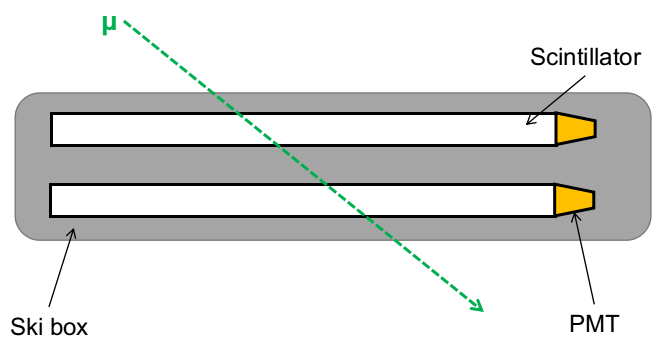
\includegraphics[width=0.75\columnwidth]{14008_config.png}
	\caption{Schematic diagram of the HiSPARC station 14008 detector set-up within the roof box/ski box.}
	\label{fig:14008_config}
\end{figure}

To protect the scintillators and \glspl{pmt}, we sandwiched a layer of high density ($\rho = 38-40$~kg~m$^{-3}$, \citet{efoam_sf38_2017}) foam, of thickness, $\Delta x = 50$~mm, between the scintillators, as can be seen on the lab work bench in Figure~\ref{fig:14008_detectors}. Upon the completed assembly of the detectors, they are placed within the roof box on the roof of the Poynting Physics building on the campus of University of Birmingham, as shown in Figure~\ref{fig:14008_ski_box}.

\begin{figure}[ht!]
	\centering
	\subfloat[Scintillators inside roof box]{
		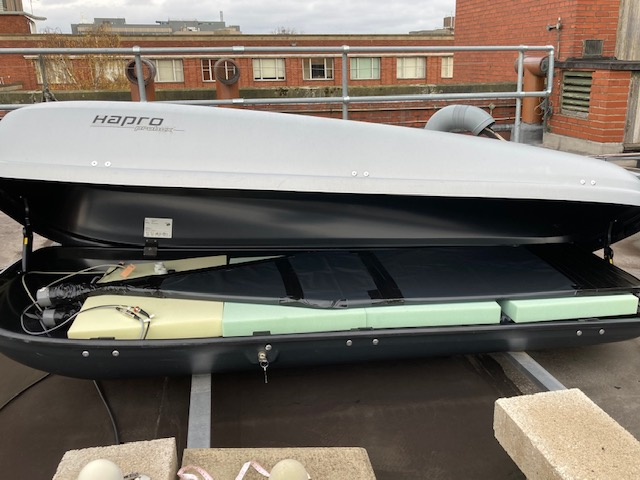
\includegraphics[width=0.48\columnwidth]{detectors_in_box.jpg}
		\label{fig:14008_detectors}}
	%\qquad
	\subfloat[Complete detector on the roof]{
		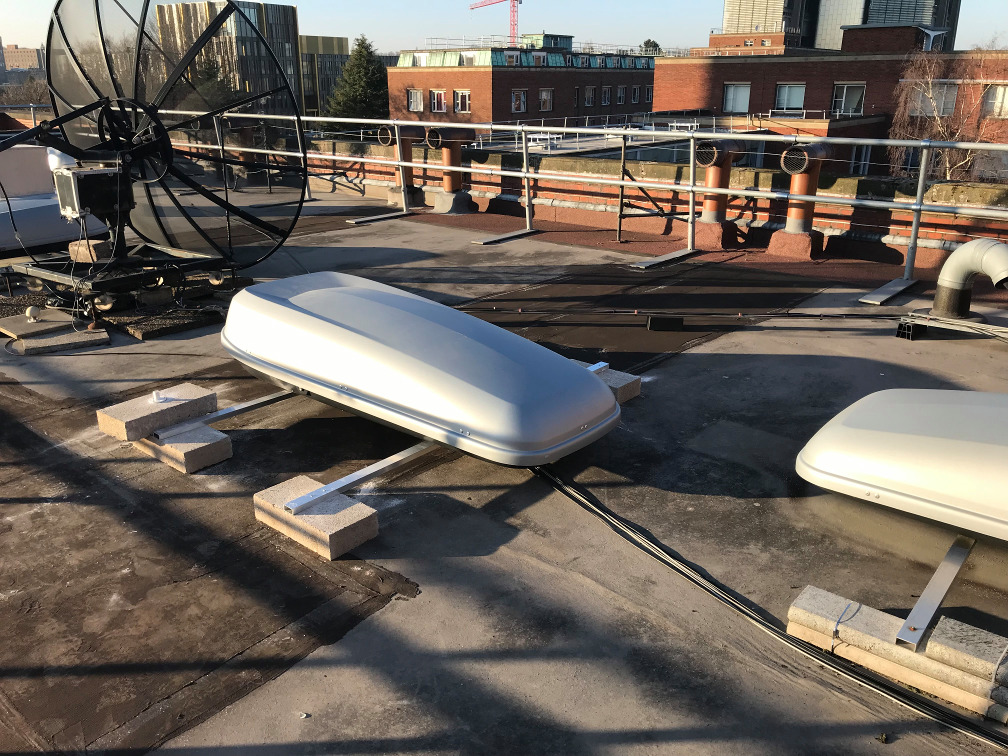
\includegraphics[width=0.48\columnwidth]{ski_box_rescaled.jpg}
		\label{fig:14008_ski_box}} \\
	
	\caption{HiSPARC 14008 assembly and configuration. (a) shows the stacked arrangement of the scintillators within the roof box, between layers of protective foam. (b) shows the complete detector on the roof of the Poynting building on the University of Birmingham campus.}
	\label{fig:HS_14008_setup}
\end{figure}


Propagating charged particles lose energy in matter. Derived from the Bethe-Bloch formula, we can estimate the amount of energy lost by a particle in a material given by:

\begin{equation}
\Delta E = \Delta x \, S \, \rho \, \cos(\theta) \, ,
\label{eq:energy_loss}
\end{equation}

where $\Delta x$ is the thickness of the material, $S$ is the stopping power of the material, $\rho$ is the density of the material, and $\theta$ is the angle the particle travels through the material from the perpendicular direction.

Each of the plastic scintillators has a thickness of $\Delta x \, = \, 2.0$~cm, and density, $\rho \, = \, 1.03$~g~cm$^{-3}$ \citep{montanus_observability_2017}. The stopping power of the scintillator for a minimum ionising particle is $S \sim 2$~MeV~g$^{-1}$~cm$^{2}$ \citep{fokkema_hisparc_2012, montanus_observability_2017}. The energy loss of a vertically incident muon in a single detector is therefore $\Delta E \sim 4$~MeV. \cite{van_dam_hisparc_2020} states the most probable energy loss of a vertically incident muon in a single scintillator is $3.51$~MeV.

 Assuming a similar stopping power as above for the foam, the muons will lose an additional $\sim 0.4$~MeV. In the complete configuration as a muon traverses two scintillators and the foam, the estimated lower limit on the energy loss by muons in the detector is $\sim 7.42$~MeV.


The standard \gls{hisparc} station set-up is such that the \glspl{pmt} are connected to the \gls{hisparc} electronics box for data acquisition. In the standard configuration, the trigger rate of events is $\sim 1$~Hz. In this stacked configuration the trigger rate is significantly higher, $\sim 70$~Hz; hence the data produced is the equivalent of approximately half of the existing \gls{hisparc} network. The network could not cope with such a large quantity of data, therefore we had to reduce the data acquired by the \gls{hisparc} box; however, we did not want to lose the full count rate of the stack detectors. To acquire the data in this set-up, we used a \gls{nim} crate, as shown in Figure~\ref{fig:14008_NIM}.

\begin{figure}[ht!]
	\centering
	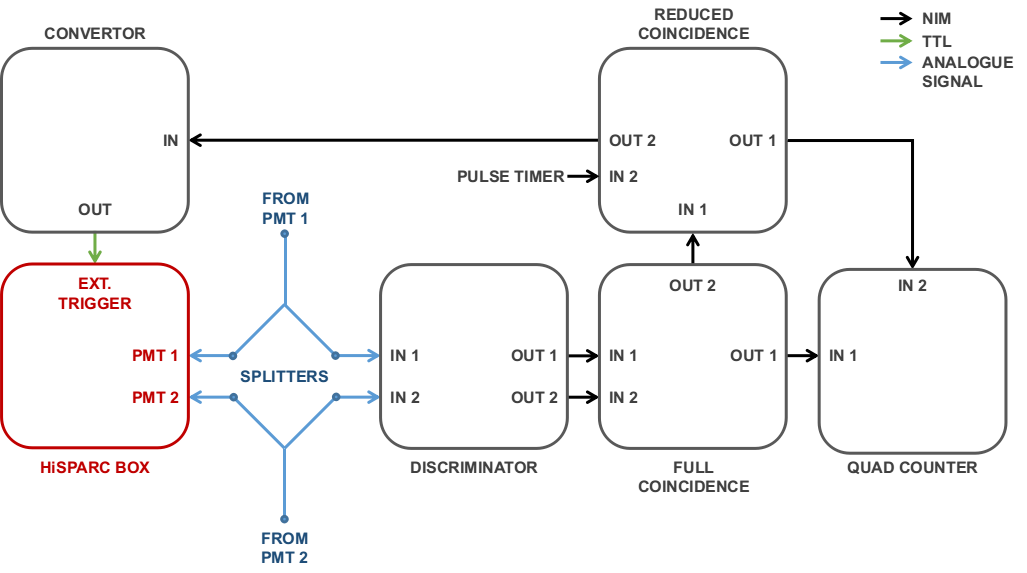
\includegraphics[width=\columnwidth]{14008_nim_config.png}
	\caption{Schematic diagram of the HiSPARC 14008 station NIM crate configuration. Black arrows depict a NIM signal; green arrows show a TTL signal; blue arrows depict a HV signal. The PMTs from the detectors are split and and this shows half the signal interfaces directly with the HiSPARC electronics box and half the signal is passed through the NIM crate for processing.}
	\label{fig:14008_NIM}
\end{figure}

The data acquisition is discussed in Section~\ref{sec:HS14008_data_acqusition}, but here we discuss the configuration of the \gls{nim} crate set-up. The \gls{hv} signal from the detector \glspl{pmt} are split using a passive, equal-split resistive splitter such that half the signal is passed to the \gls{hisparc} electronics box and half the signal is passed through the \gls{nim} crate. The signal which is passed through the \gls{nim} crate is first passed into a discriminator module (CAEN model N845) to only record signals that have an amplitude greater than the trigger threshold. Due to the equal-balance resistive splitter the \gls{hv} signal is reduced in amplitude by a factor of 2; we used a discriminator threshold of $-35$~mV, i.e. half of the \gls{hisparc} high threshold.

The discriminator outputs two \gls{nim} signals which are connected to the first coincidence module (LeCroy model 622). This records every coincidence between the two \glspl{pmt} and the output from this module is directed to a \gls{nim} quad counter/timer module (ORTEC model 974). One channel of the \gls{nim} counter records the full coincidences from the first coincidence module.

A second terminal in the coincidence module was used to record a reduced count rate. This used a pulse timer (CAEN model 2255B) to create a gate signal with a $\sim 1\%$ duty cycle (gate width = $45.0 \, \upmu\mathrm{s}$ and repeat period = $4.86$~ms). The coincidence between the full coincidence signal and the pulse timer gate ensures that the full count rate is reduced by a factor of $\sim 100$. One output from this coincidence module is passed to the \gls{nim} counter, where it counts the reduced coincidences. The second output from the coincidence module is directed through a \gls{nim}-to-\gls{ttl} convertor and the output from this is used as an external trigger signal to trigger the acquisition of data by the \gls{hisparc} electronics box. This acquires the counts directly from the \glspl{pmt}.

[discussion, and also probably use a table, to discuss the delays introduce by the NIM crate...]


%%%%%%%%%%%%%%%%%%%%%%%%%%%%%%%%%%%%%%%%%%%%%%%%%%%%%%%%%%%%%%%%%%%%%
\subsection{Calibration}

When setting up the HiSPARC station, it was required to set several operating parameters for the detectors and the HiSPARC electronics box. One such setting was the \gls{pmt} operating voltage. Each of the detector \glspl{pmt} needs to be powered with a high enough operating voltage such to provide an amplified signal, but not too high such as to over-amplify the noise.

In general, the \glspl{pmt} has an advised operating voltage of around 700~V \citep{fokkema_hisparc_2019}; however, best practise is to operate the \gls{pmt} at the plateu region, whereby the counts/voltage no longer increases. As can be seen from Figure~\ref{fig:PMT_cal}, neither of the \glspl{pmt} have clear plateau regions, hence there was no obvious \gls{pmt} set point.

The HiSPARC installation manual does, however, suggest to tune the \gls{pmt} voltages such that the singles rates for each detector meet the following criteria: singles rate of 100--130 Hz for signal above the high trigger threshold, and singles rate of $<$400 Hz for signal above the low trigger threshold \citep{fokkema_hisparc_2019}.

In order to calibrate the \glspl{pmt} to the correct level, we measured the singles rates above the high and low thresholds as a function of \gls{pmt} operating voltage, as is shown in Figure~\ref{fig:PMT_cal} [UPDATE THIS PLOT...!!!!]. The voltage calibration plot shows drastically the different performances one can get from different \glspl{pmt}, therefore it is necessary to treat each \gls{pmt} individually when calibrating.

\begin{figure}[ht!]
	\centering
	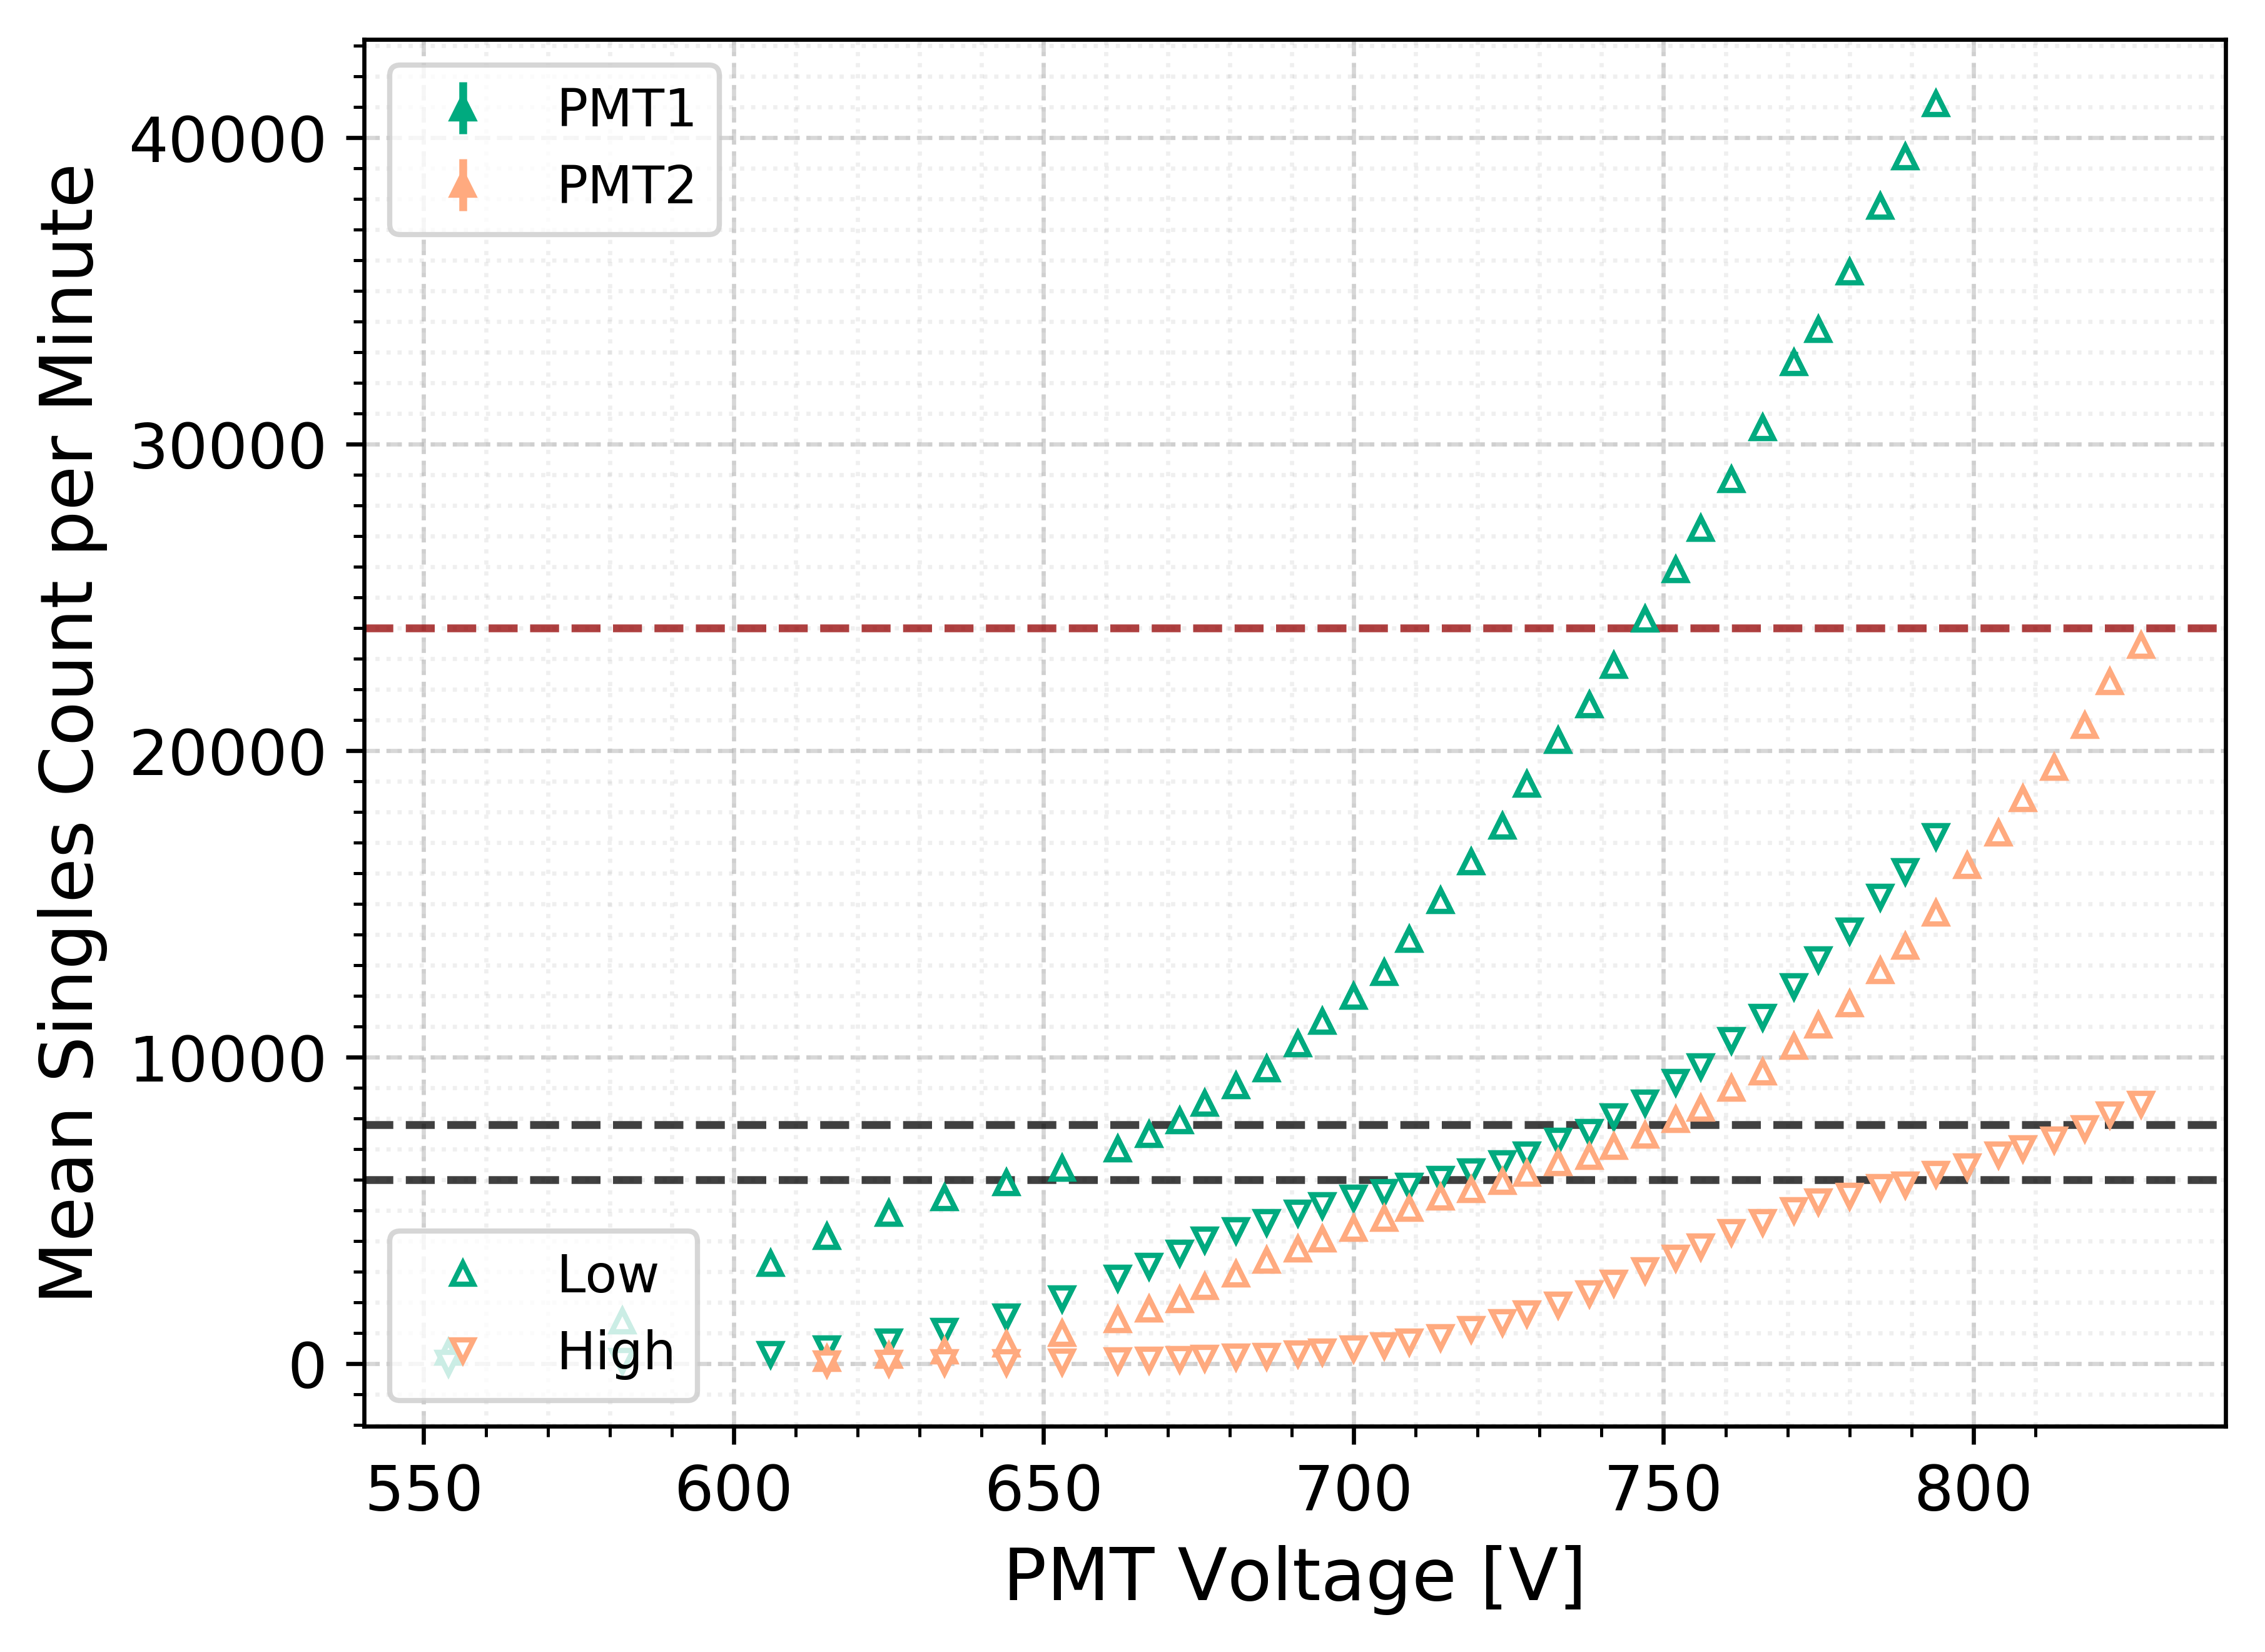
\includegraphics[width=0.8\columnwidth]{both_PMTs_post_NIM.png}
	\caption{Voltage calibration curve for the PMTs of station 14008. The upper, red-dashed line indicates the upper limit for the low threshold singles rate (400 Hz), and the lower 2, black-dashed lines indicate the upper and lower bounds for the high threshold singles rate (100--130 Hz).}
	\label{fig:PMT_cal}
\end{figure}




%%%%%%%%%%%%%%%%%%%%%%%%%%%%%%%%%%%%%%%%%%%%%%%%%%%%%%%%%%%%%%%%%%%%%
\subsection{Monitoring Temperature}

In Chapter~\ref{chap:HiSPARC}, we suspected that the singles count rates (and thus event count rates also) were affected by the temperature of the \gls{pmt} within the HiSPARC roof-boxes.

Some of the existing HiSPARC stations monitor local temperature however none measure the temperature of the \gls{pmt} within the roof box; therefore the temperature of the PMT itself is unknown, and thus we cannot account for the thermal noise. When building this new HiSPARC station, a temperature sensor was placed into the roof box which allowed us to monitor the temperature.

Figure~\ref{fig:temperature_sensor_circuit} shows the schematic for the temperature sensor. We used the DS18B20 temperature sensor with the one-wire telemetry protocol, which used a single wire to transmit the temperature readings to the microcontroller; the microcontroller used was a Raspberry Pi 4 (see Section~\ref{sec:HS14008_data_acqusition}). Three wires were used for the operation of the DS18B20: constant current voltage, ground, and data. The temperature is read on a 10-second cadence and is recorded in degrees Celsius with a precision of $0.001^{\circ}$~C. 

\begin{figure}[htbp!]
	\centering
	\subfloat[Circuit diagram]{
		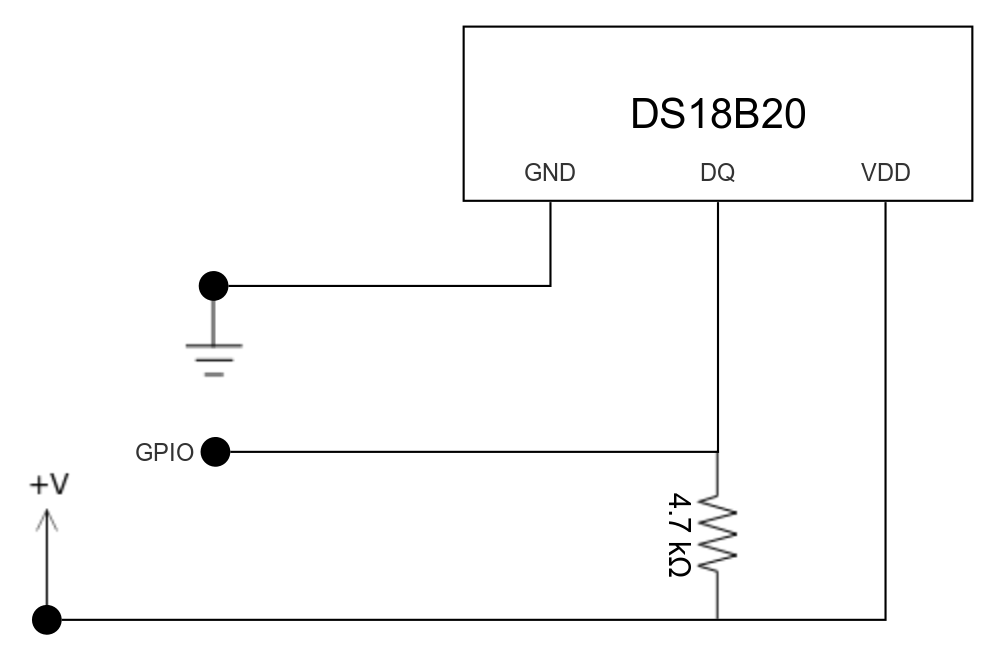
\includegraphics[width=0.6\columnwidth]{HS_14008_temp_circuit.png}
		\label{fig:temperature_sensor_circuit}}
	
	%\qquad
	\subfloat[Sensor within roof box]{
		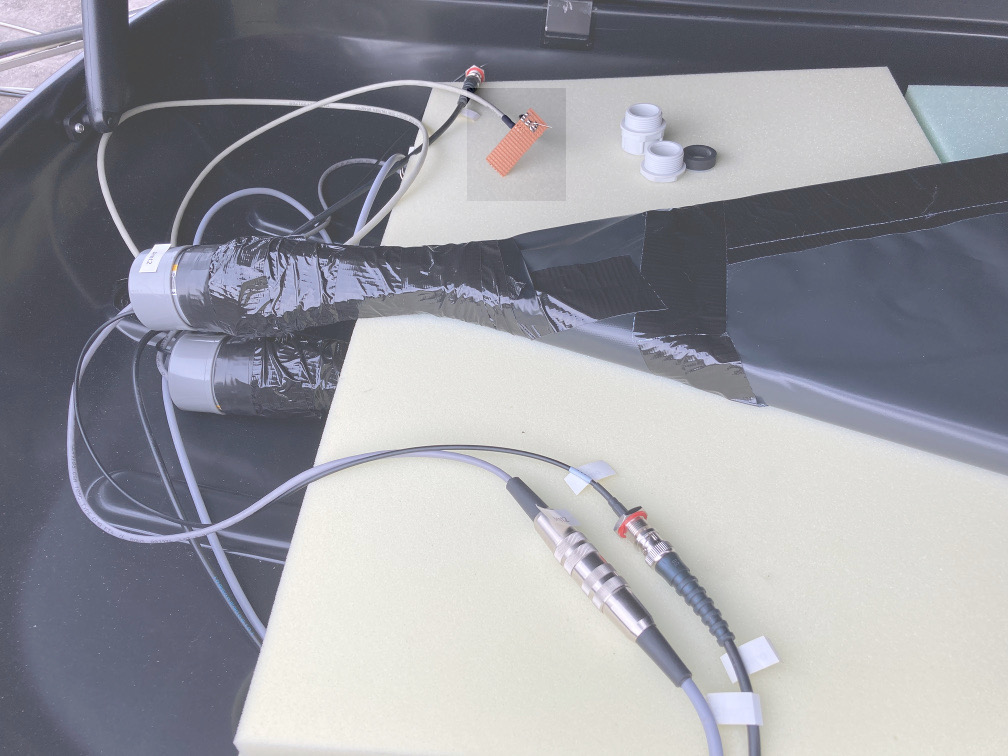
\includegraphics[width=0.55\columnwidth]{temperture_sensor_rescaled.jpg}
		\label{fig:temperature_sensor_in_box}} \\
	
	\caption{(a) Schematic diagram of the DS18B20 temperature sensor circuit, whereby the voltage, ground, and GPIO interfaces connect directly into pins of the Raspberry Pi board. (b) the sensor within the roof boxes, located by the PMTs. The temperature sensor is soldered into the circuit board in the top-middle of the image.}
	\label{fig:temperature_sensor}
\end{figure}



%%%%%%%%%%%%%%%%%%%%%%%%%%%%%%%%%%%%%%%%%%%%%%%%%%%%%%%%%%%%%%%%%%%%%
\subsection{Data Acquisition}
\label{sec:HS14008_data_acqusition}

The new \gls{hisparc} station uses two methods of data acquisition. The singles data and reduced coincidences data are acquired using the typical \gls{hisparc} data acquisition software, but the full coincidences, reduced coincidences, and the temperature data are all acquired by a Raspberry Pi 4. This was done as it allowed us to store the full coincidences data. A schematic diagram showing the interfaces between the Raspberry Pi and the other hardware is shown in Figure~\ref{fig:14008_RP4}.

\begin{figure}[ht!]
	\center
	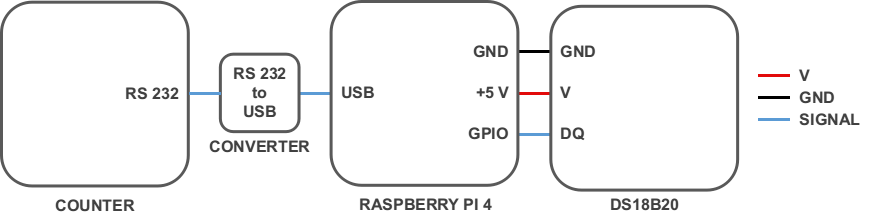
\includegraphics[width=0.8\columnwidth]{14008_data_acq_config.png}
	\caption{Schematic diagram of the HiSPARC station 14008 data acquisition interfaces.}
	\label{fig:14008_RP4}
\end{figure}


The Raspberry Pi 4 was used to control the data acquisition by running a Python script. The scripts configured the hardware and output the coincidences data from the \gls{nim} counter and the temperature data from the DS18B20 sensor to local files on the Raspberry Pi. Both the coincidences and temperature data are recorded on a 10 second cadence.

Each new day generates a separate file for the coincidences data and temperature data. Within the coincidence files there are no headers and the data begins from line 1. The files contain four columns and the data stored in each column is listed in Table~\ref{tab:HS_14008_coincidences_data}.

\begin{table}[ht!]
	\begin{center}
		\caption{Variables stored in the coincidences files of the HiSPARC 14008 instrument.}
		\label{tab:HS_14008_coincidences_data}
		\begin{tabular}{cp{0.2\linewidth} lp{0.35\linewidth} cp{0.3\linewidth} cp{0.35\linewidth}}
			\hline 
			{\bf Column} & {\bf Item} & {\bf Unit} & {\bf Type} \\ 
			\hline 
			\multirow{2}*{0} & \multirow{2}*{Time Stamp} & YYYY\_MM\_DD & \multirow{2}*{String}  \\ 
			  &  & HH:MM:SS.ffffff & \\ 
			1 & Time*  & Decisecond & Integer, eight digits, zero padded \\ 
			2 & Cumulative Reduced Count* & Counts & Integer, eight digits, zero padded \\ 
			3 & Cumulative Full Count* & Counts & Integer, eight digits, zero padded \\ 
			\hline 
		\end{tabular} 
	\end{center}
	* Since restart
\end{table}

The \gls{nim} counter records the cumulative coincidences count, therefore the reduced and full data stored are also cumulative and thus when reading the data, one must ensure that the difference is calculated between timestamps. In the event of hardware or software failure, or a reboot of the Raspberry Pi, when the Python script re-runs the \gls{nim} counter restarts all values from 0. When reading a file, one must ensure that checks are in place to handle any restarts from zero appropriately, such that no negative counts are calculated from one timestamp to the next during a restart.

Within the temperature files, there are also no headers and the data begins from line 1. The columns in the data file are outlined in Table~\ref{tab:HS_14008_temperature_data}.

\begin{table}[ht!]
	\begin{center}
		\caption{Variables stored in the temperature files of the HiSPARC 14008 instrument.}
		\label{tab:HS_14008_temperature_data}
		\begin{tabular}{c l l l}
			\hline 
			{\bf Column} & {\bf Item} & {\bf Unit} & {\bf Type} \\ 
			\hline 
			\multirow{2}*{0} & \multirow{2}*{Time Stamp} & YYYY\_MM\_DD & \multirow{2}*{String}  \\ 
			  &  & HH:MM:SS.ffffff & \\ 
			1 & Temperature & $^\circ$C & Floating point \\ 
			\hline 
		\end{tabular} 
	\end{center}
\end{table}


The data is stored locally, but it is also stored on the University of Birmingham particle physics servers as a back-up\footnote{Disk location: /disk/moose/general/epesv001/datadisk/147.188.46.117\_hisparc\_pi/}. Access to the data is not necessarily open, and to request access, one should contact the System Administrator for the Particle Physics Group Computing Facilities.

The reduced coincidences data are acquired using the \gls{hisparc} data acquisition software and are stored within the \gls{hisparc} servers. The \gls{hisparc} servers record this data as the events and the data can be acquired using the methods described in Section~\ref{sec:HS_data}.




[What is the width of the signals generated by the NIM crate? Is it more or less than the approx. 25ns FWHM of the pulses..? Then relate that to: "The pulse width, Tw, is important only insofar as it determines the maximum rate of pulses that may be represented by the pulse train, since pulses which occur more frequently than 1/Tw cannot be resolved"...]



[a few statements on the availability of the data... i.e. it's generally ok and a complete set beyond Feb 2020, but many interruptions due to the pandemic... After around Sept 2020 the data becomes more reliable...]



%%%%%%%%%%%%%%%%%%%%%%%%%%%%%%%%%%%%%%%%%%%%%%%%%%%%%%%%%%%%%%%%%%%%%
\subsection{Monitoring Pressure}

As with the previous chapter, it was still necessary to account for the barometric effect on the muon count rate, for both the singles data and the full and reduced coincidences data. To monitor the pressure, a nearby station was used, which is part of the \gls{midas} database, and acquired from the \gls{stfc} and \gls{nerc} \gls{ceda} archive.

The \gls{midas} station used is the nearest pressure monitor to the \gls{hisparc} and provides a robust measure of the local atmospheric pressure. The pressure is measured at the \gls{midas} station level and a correction for altitude is not applied. The station is located in Coleshill, Warickshire (ID: 19187), nearby Birmingham International Airport, $\sim 20$~km from the HiSPARC detectors; we believe the pressure variation is small over this distance.

The pressure data is recorded on a 1-hour cadence in units of hPa, with a precision of 0.1~hPa. The time variation of pressure is slow; hence, we linearly interpolated the data to provide a 1-minute sample.


%%%%%%%%%%%%%%%%%%%%%%%%%%%%%%%%%%%%%%%%%%%%%%%%%%%%%%%%%%%%%%%%%%%%%
%%%%%%%%%%%%%%%%%%%%%%%%%%%%%%%%%%%%%%%%%%%%%%%%%%%%%%%%%%%%%%%%%%%%%
\section{Methodology}\label{sec:HS_14008_methods}

\subsection{Atmospheric Corrections}

Using the theory outlined in Section~\ref{sec:HS_P_corr} we were able to perform the barometric correction of the singles data and coincidences data, whereby a linear fit was made using the model defined by equation~(\ref{eq:presscorr3}). ...

After considerate review of the method of temperature correction, the method also discussed in Chapter~\ref{chap:HiSPARC} was used, i.e. the linear relationship; however, the method was tweaked slightly. The steps for correcting for the effect of temperature were:

\begin{itemize}
	\item{To remove the long--term temperature trend over a month of data, the \gls{cr} and temperature data were smoothed using a 24-hr moving mean. Using the linear relationship defined by equation~(\ref{{eq:presscorr3}}), changing pressure to temperature, the long--term temperature relationship was fit and was removed from the data.}

	\item{After removing the long--term temperature relationship, for each day the temperature correction was applied again to remove the daily variations. During the fit to the data the values of $N_0$ and $T_0$ used we the de-trended 24-hr smoothed data.}
\end{itemize}

This was done, as during the initial temperature corrections here, it was found that without removing the long--term temperature relationship there was still some long--term covariance between the temperature and the \gls{cr} count. In addition, without using the de-trended, 24-hr smoothed data as the value for the values of $N_0$ and $T_0$, we found that after the corrections, there existed jumps between days; this method ensure that there is a smooth transition in the corrected data between days.


\subsection{Observations}\label{sec:HS_14008_method_obs}

The probability distribution of the number of counts in a fixed interval of time follows the Poisson distribution and is defined by:

\begin{equation}
P(k; \, \lambda) = \frac{\lambda^k \, e^{-\lambda}}{k!} \, ,
\label{eq:poisson_PDF}
\end{equation}
%
where $k$ is the number of events, which is always an integer, and $\lambda$ is the mean value of the number of events per interval, i.e. the expected number. Under the Poisson distribution, the mean and the variance are both equal to $\lambda$. For a large value of $\lambda$, the Poisson distribution can be approximated with a Gaussian distribution having mean, $\lambda$, and standard deviation, $\sqrt{\lambda}$.

The Poisson distribution is also additive such that if two variables, $n_1$ and $n_2$, follow Poisson distributions, with mean values $\lambda_1$ and $\lambda_2$, respectively, then the sum also follows a Poisson distribution:

\begin{equation}
P(n; \, \lambda_1, \lambda_2) = P(n; \, \lambda_1 + \lambda_2) \, ,
%\sum_{min}^{max} P(k; \, \lambda) P(k; \, \lambda) =
%p. 40 in Lista, L. (2016) 
\label{eq:poisson_additive_PDF}
\end{equation}
%
where $n = n_1 + n_2$.

Using this information, it was possible to use a sampling algorithm to determine the mean level and noise of the \gls{hisparc} 14008 station's data. With this knowledge artificial data was created, to simulate the detector's response to space weather events. 

Artificial data was generated using the method discussed in Appendix~\ref{app:GLE_sims}
%[probs = 1-sts.poisson.cdf(x-1, mu)]
%[bin_probs = [1 - sts.binom.cdf(1-1, N, p_i) for p_i in probs]]

During the analysis of simulated data, we used a series of statistical tests to determine whether we could observe the injected \glspl{gle}. We can use the fact that count data follow a Poisson distribution to compute the probability of statistically significant spikes in the data. The Poisson cumulative distribution function is given by:

\begin{equation}
F(k; \, \lambda) = \sum_{i=0}^{k}  \frac{\lambda^i \, e^{-\lambda}}{i!} \, ,
\label{eq:poisson_CDF}
\end{equation}


Using this expression, the probability that a cadence observes $k$ or more events, given the mean level, $\lambda$, is therefore given by: 

\begin{equation}
p(k) = 1 \, - \, F(k; \, \lambda) \, .
\label{eq:poisson_SF}
\end{equation}

The probability that we fail to observe a cadence with $k$ or more events is: $1 \, - \, p(k)$; thus the probability of failing to observe any cadence with $k$ or more events in $N$-cadences is $[1 \, - \, p(k)]^N$. Therefore the probability to find at least one event at or above $\lambda$ in N-cadences is:

\begin{equation}
p_N = 1\, - \, [1 \, - \, p(\lambda)]^N \, ,
\label{eq:poisson_p_N}
\end{equation}
%
where a low value for $p_N$ indicates that the observed event is considered statistically significant.

This can be generalised using the cumulative binomial distribution. The probability of finding at least $r$ occurrences in $N$-cadences at or above $k$, given the mean level, $\lambda$, is given by equation~(\ref{eq:poisson_binom_CDF}), which is equal to equation~(\ref{eq:poisson_p_N}) when $r=1$,

\begin{equation}
p[r; p(k), N] = \sum_{r=r}^{N} \binom{N}{r} \, p(k)^r \, [1 \, - \, p(k)]^{N-r} \, .
\label{eq:poisson_binom_CDF}
\end{equation}

By applying equation~(\ref{eq:poisson_binom_CDF}) to the data, we were able to test whether there were any significant events. Again, a low value for $p[r; p(\lambda), N]$ indicates that the event is statistically significant.


Another frequentist test that was used uses the assumption that the Poisson distribution tends towards a Gaussian distribution when the mean value is sufficiently large. An excess in counts, compared to the mean value, can be quantified as:
%s = x - mu
%z = s / std

\begin{equation}
s = k - \lambda \, ,
\label{eq:poisson_excess}
\end{equation}
%
where $s$ is the excess in the signal, $k$ is the measured signal and $\lambda$ is the expected value, or background signal. The significance can then be approximated by:

\begin{equation}
Z = \frac{s}{\sigma} \, ,
\label{eq:poisson_significance}
\end{equation}
%
where $\sigma$ is the expected standard deviation, which for a Poisson distribution is $\sqrt{\lambda}$. In this work we used both $Z = 3$ and $Z = 5$ significance levels to determine the existence of excess signals.

As a further test we also analysed re-sampled versions of the artificial data. This allowed us to reduce the Poisson noise, with the ambition of reducing the noise such to allow us to observe lower amplitude space weather events. We also ran the statistics tests on 1-minute and 5-minutes averages of the artificial data. The statistical tests were run under the same underlying principals, however instead of using the Poisson cumulative distribution in equation~(\ref{eq:poisson_SF}), we instead used the Gaussian cumulative distribution for the averaged data with mean, $\mu = \lambda$, and standard deviation, $\sigma = \sqrt{\mu/n}$, where $n$ represents the number of data points used in the average. Similarly, using the Gaussian distribution with mean, $\mu = \lambda$, and  standard deviation, $\sigma = \sqrt{\mu/n}$, in equation~(\ref{eq:poisson_significance}).



%%%%%%%%%%%%%%%%%%%%%%%%%%%%%%%%%%%%%%%%%%%%%%%%%%%%%%%%%%%%%%%%%%%%%
%%%%%%%%%%%%%%%%%%%%%%%%%%%%%%%%%%%%%%%%%%%%%%%%%%%%%%%%%%%%%%%%%%%%%
\section{Atmospheric Corrections}\label{sec:HS_14008_atmospheric_correction}

%%%%%%%%%%%%%%%%%%%%%%%%%%%%%%%%%%%%%%%%%%%%%%%%%%%%%%%%%%%%%%%%%%%%%
\subsection{Barometric Correction}\label{sec:HS_14008_P_corr}


Using the theory outlined in Section~\ref{sec:HS_P_corr} we were able to perform the barometric correction between the 1-minute interpolated pressure data and 1-minute averaged coincidences and singles data.

[show the plot of the correction over a month...]


\begin{figure}[ht!]
	\centering
	\subfloat[Comparison between singles and pressure]{
		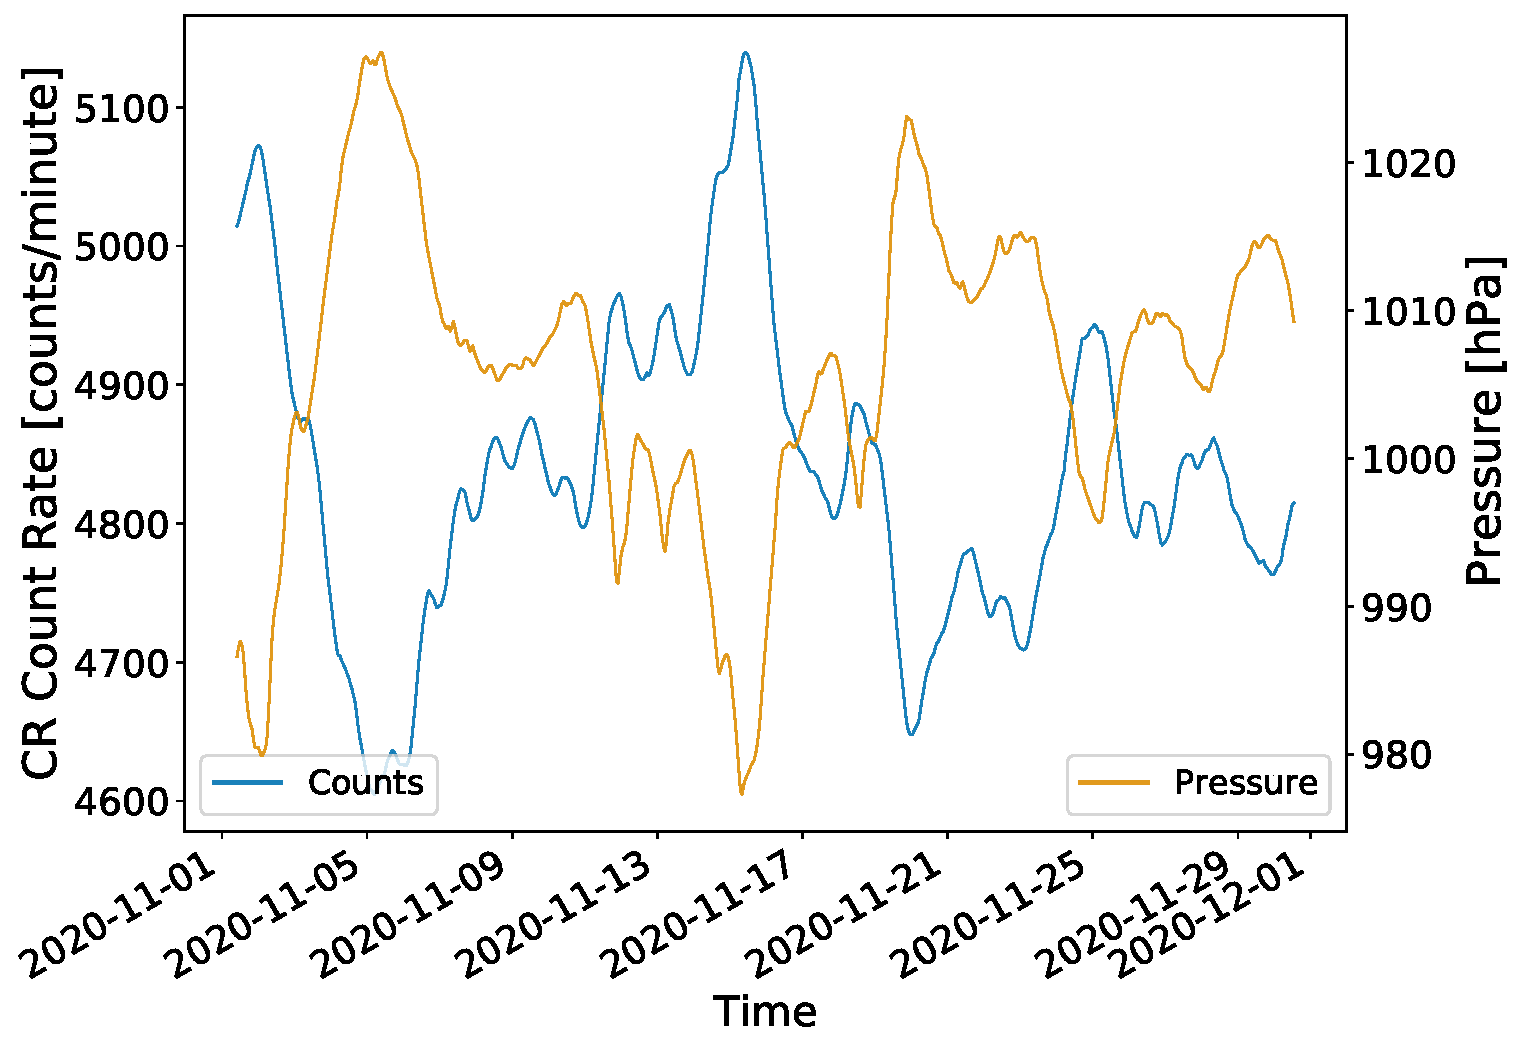
\includegraphics[width=0.48\columnwidth]{CR_v_P.pdf}
		\label{fig:HS_14008_CRvP}}
	%\qquad
	\subfloat[Correlation between singles and pressure]{
		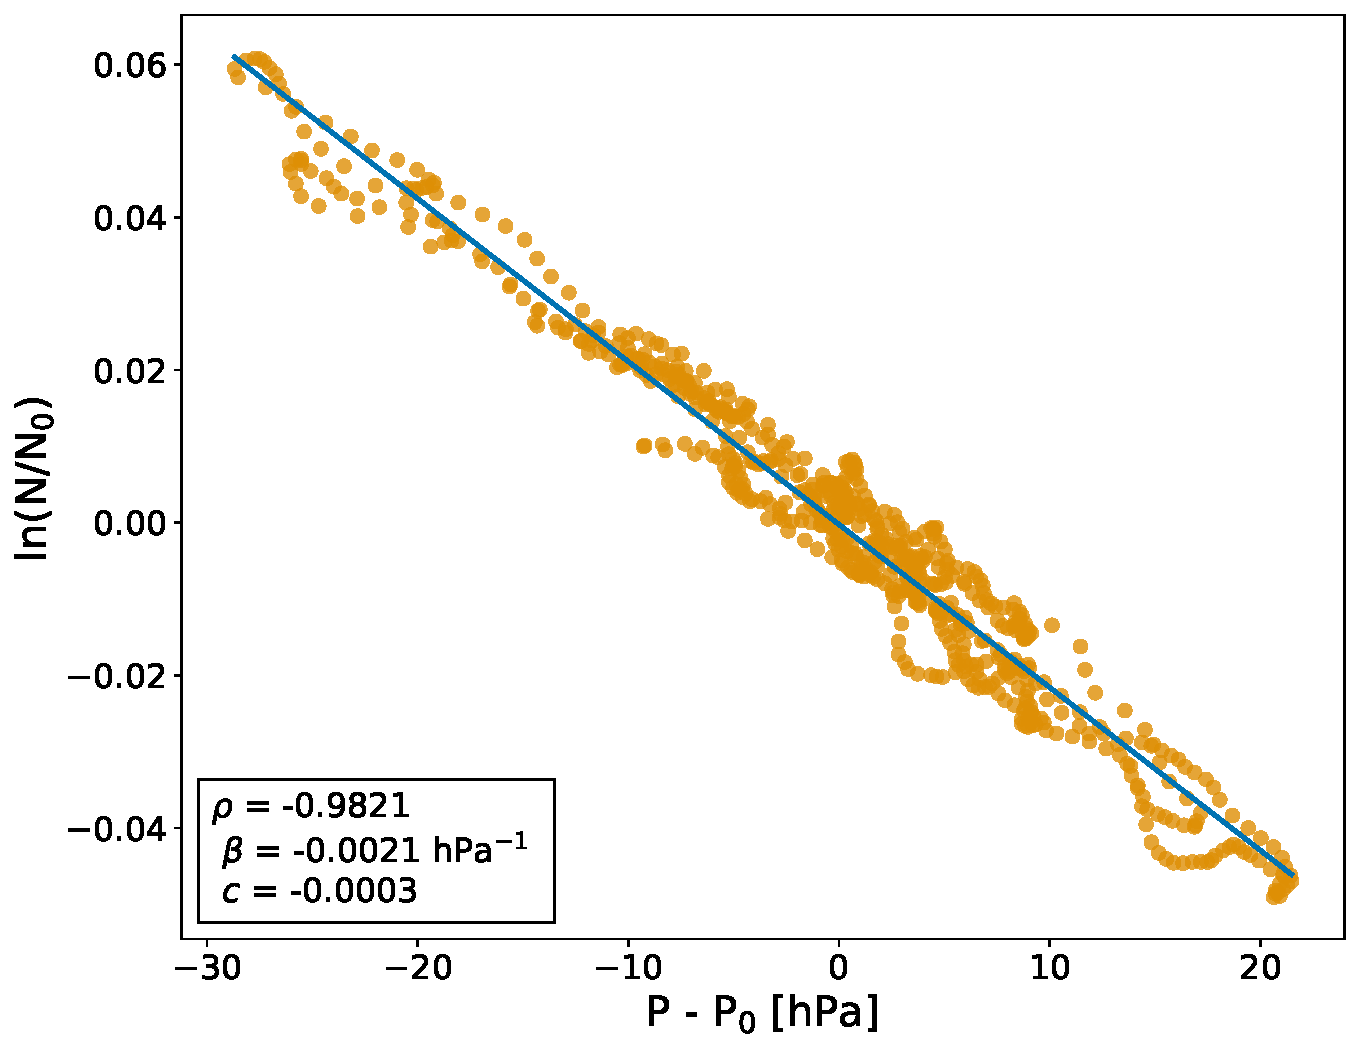
\includegraphics[width=0.48\columnwidth]{fit_CR_v_P.pdf}
		\label{fig:HS_14008_beta}} \\
	
	\caption{The relationship between the ... (a) shows the ... and pressure data; (b) shows the correlation between the singles counts and pressure, and the fitted line to calculate the correction coefficient.}
	\label{fig:14008_CR_V_P_corr}
\end{figure}


[show a before vs after plot too...]


\begin{figure}[ht!]
	\centering
	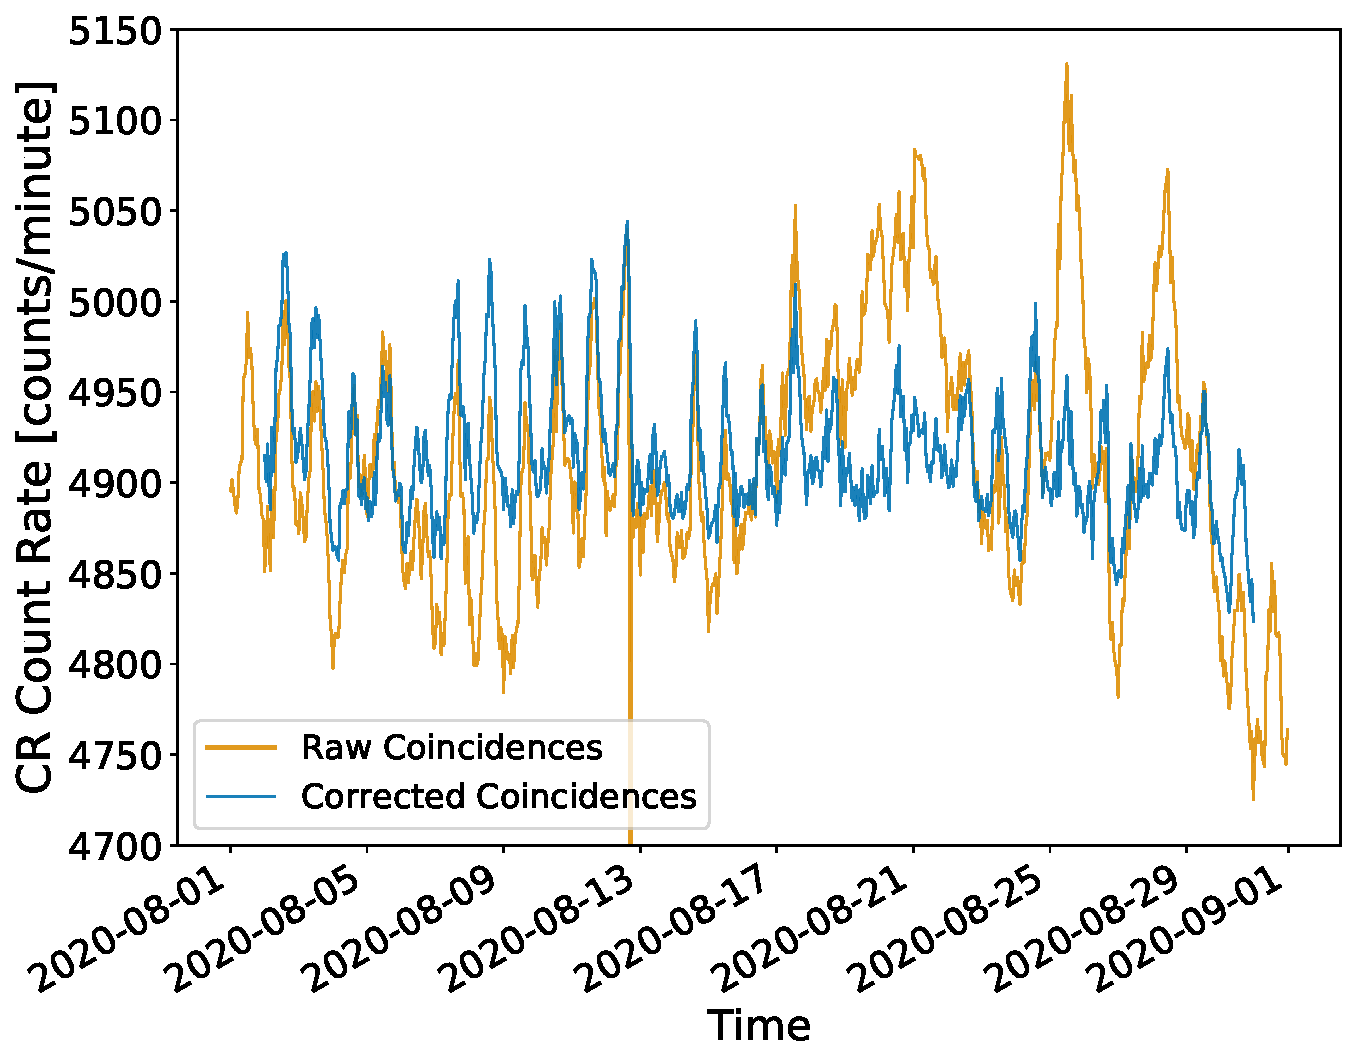
\includegraphics[width=0.75\columnwidth]{raw_vs_corrected_coincidences.pdf}
	\caption{Showing the coincidence data before (orange line) and after(blue line) the barometric correction.}
	\label{fig:HS_14008_corrected_coincidences}
\end{figure}



%%%%%%%%%%%%%%%%%%%%%%%%%%%%%%%%%%%%%%%%%%%%%%%%%%%%%%%%%%%%%%%%%%%%%
\subsection{Temperature Correction}\label{sec:HS_14008_T_corr}

One can see the relationship between the singles rates and the temperature in Figure~\ref{fig:HS_14008_temperature_vs_CR}...

\begin{figure}[ht!]
	\centering
	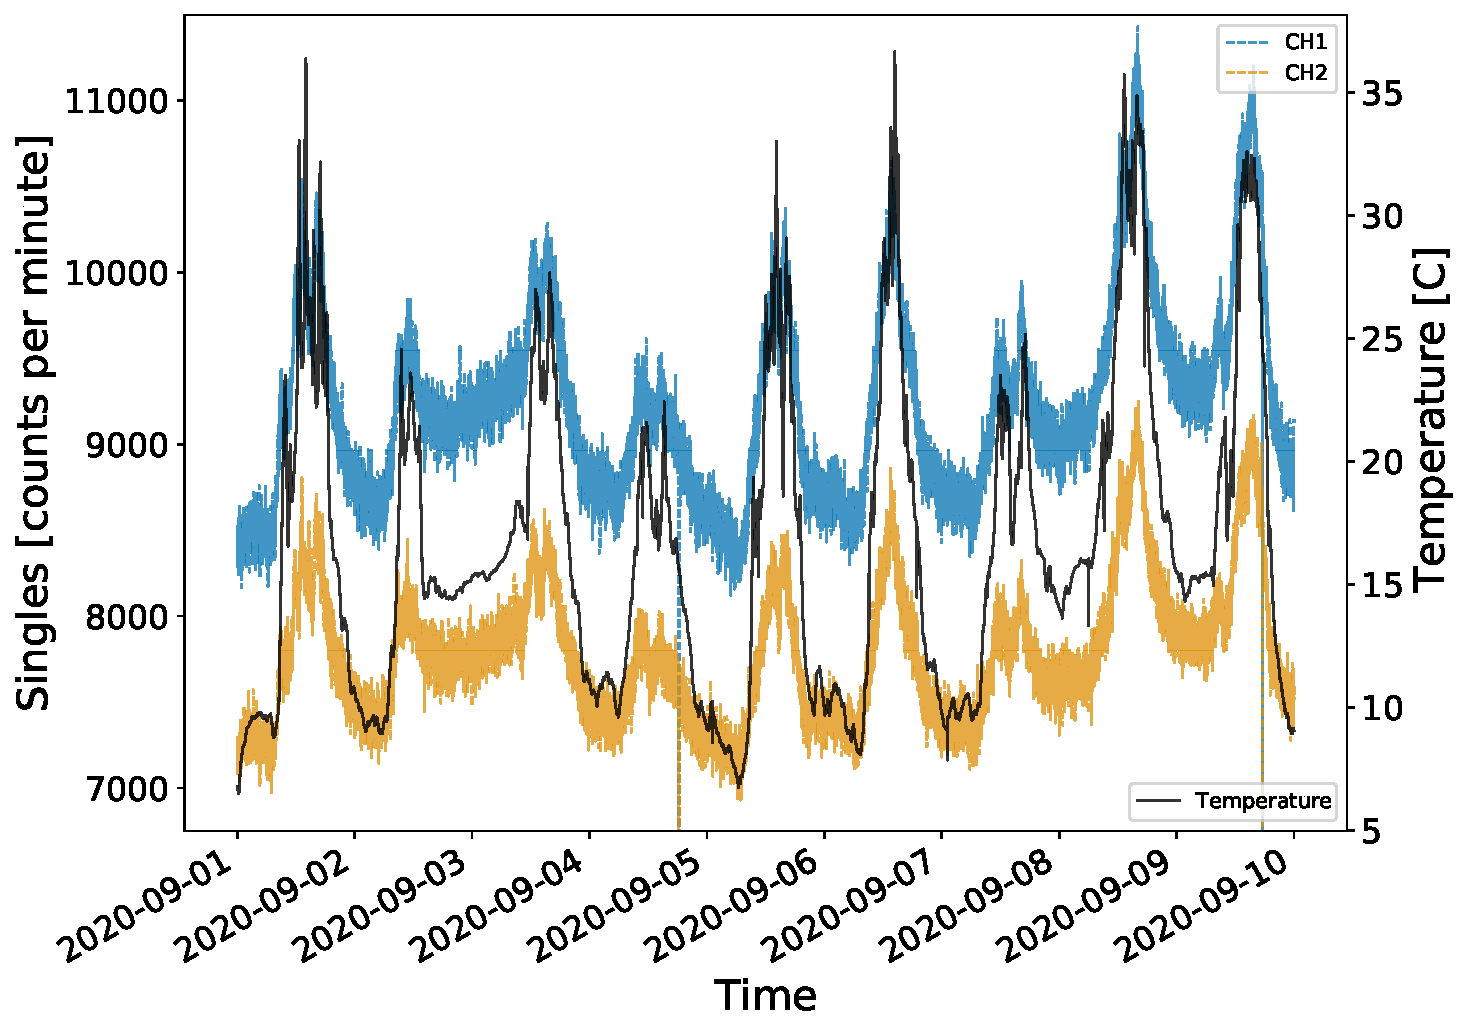
\includegraphics[width=0.75\columnwidth]{HS_14008_CR_v_T_sept2020.pdf}
	\caption{...}
	\label{fig:HS_14008_temperature_vs_CR}
\end{figure}




\begin{figure}[ht!]
	\centering
	\subfloat[...]{
		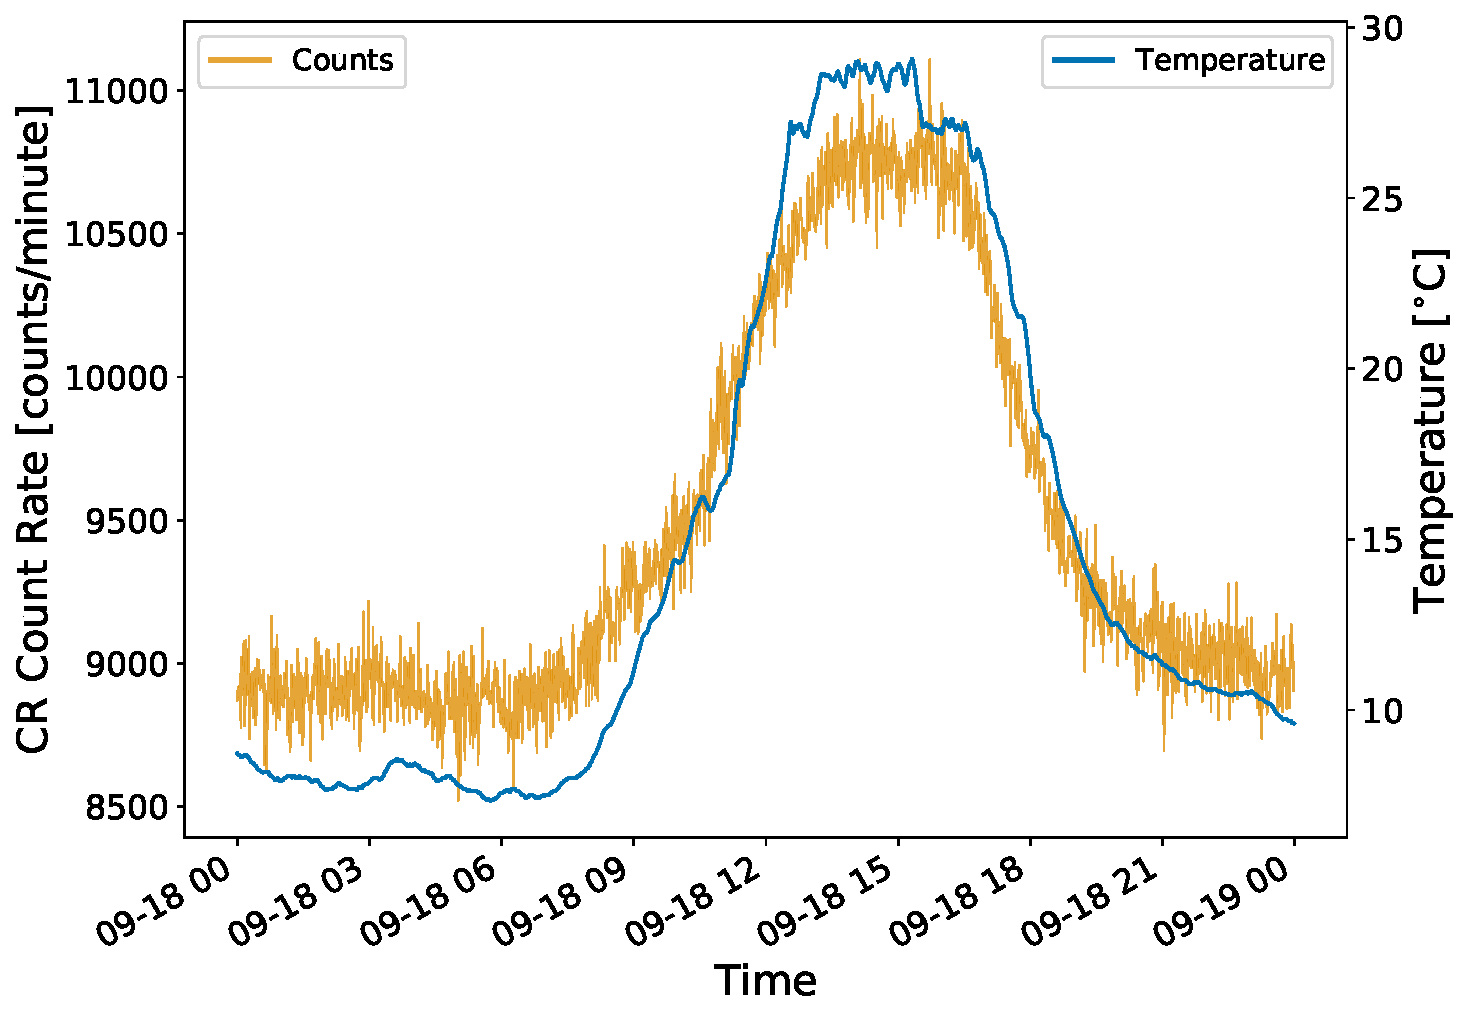
\includegraphics[width=0.48\columnwidth]{CR_v_T.pdf}
		\label{fig:HS_14008_CRvT}}
	%\qquad
	\subfloat[Correlation between singles and temperature]{
		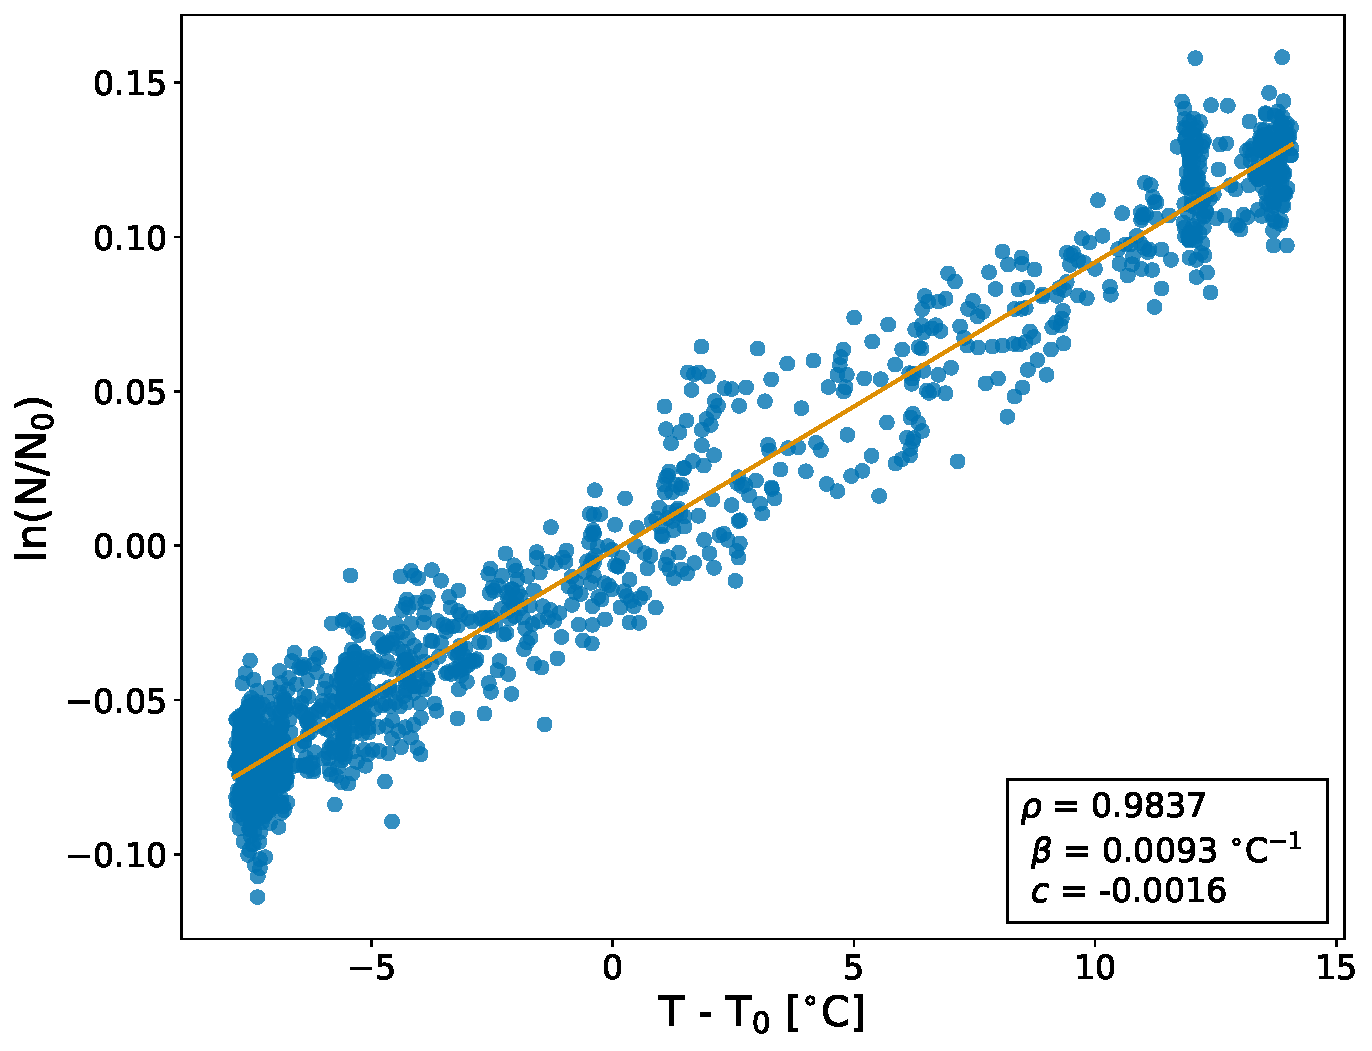
\includegraphics[width=0.48\columnwidth]{fit_CR_v_T.pdf}
		\label{fig:HS_14008_alpha}} \\
	
	\caption{The relationship between the ... (a) shows the ... and temperature data; (b) shows the correlation between the singles counts and temperature, and the fitted line to calculate the correction coefficient.}
	\label{fig:14008_CR_V_T_corr}
\end{figure}


An additional benefit of the temperature monitor at station 14008 is that it is suitable for providing an estimate of the temperature inside the roof-boxes of stations 14001, which is located on the same roof.... [show figure of the singles for both stations and the temperature!]


[Note: temperature correction doesn't work/not necessary on the coincidences but it is necessary on the singles rates!]





%%%%%%%%%%%%%%%%%%%%%%%%%%%%%%%%%%%%%%%%%%%%%%%%%%%%%%%%%%%%%%%%%%%%%
%%%%%%%%%%%%%%%%%%%%%%%%%%%%%%%%%%%%%%%%%%%%%%%%%%%%%%%%%%%%%%%%%%%%%
\section{Results}\label{sec:HS_14008_results}

%%%%%%%%%%%%%%%%%%%%%%%%%%%%%%%%%%%%%%%%%%%%%%%%%%%%%%%%%%%%%%%%%%%%%
%%%%%%%%%%%%%%%%%%%%%%%%%%%%%%%%%%%%%%%%%%%%%%%%%%%%%%%%%%%%%%%%%%%%%
\subsection{Observations}\label{sec:HS_14008_observations}

From the \gls{corsika} simulations in Chapter~\ref{chap:HiSPARC}, we predicted a ground level muon rate passing through a single \gls{hisparc} detector of $\sim 85 \, \upmu/\mathrm{s}$ (for non-vertical, i.e. $70^\circ$ acceptance cone simulations), and $160 \, \upmu/\mathrm{s}$ (for vertical simulations). These rates were comparable to the generally accepted, average ground level muon flux on the order of $\sim 70 \, \mathrm{m}^{-2}\,\mathrm{s}^{-1}\,\mathrm{sr}^{-1}$ \citep{cecchini_cosmic_2000, blackmore_terrestrial_2015, pereira_ground_2020, particle_data_group_review_2020}.

%(do this by intergrating under curve, using 70-degre half-angle cone for solid angle, and area of 0.5m2)
% i.e. in python doing doing:
% where df contains the alpha and proton diff fluxes
% v = scipy.integrate.simps(df_a_v[1]+df_p_v[1], df_a_v.index.values)
% sr = 4*np.pi*(np.sin(np.deg2rad(70/2)))**2
% area = 0.5
% rate_v = v*sr*area

In Figure~\ref{fig:corrected_coinciences} we show the full coincidence count for a typical day. In this plot we can see the diurnal effect. The diurnal effect measured here induced a variation in the \gls{cr} count between $\sim 1-2 \%$, which is larger than the $\sim 0.5 \%$ diurnal variation, discussed in the literature \citep{mishra_study_2007, mishra_cosmic_2008, dubey_cosmic_2016, thomas_decadal_2017}, but is significantly lower than the variation observed in the \gls{hisparc} events and singles data in Chapter~\ref{chap:HiSPARC}. For any given epoch, the diurnal effect can be removed, if necessary, by removing the trend of a 12-hour smoothed data set, which is also shown in Figure~\ref{fig:corrected_coinciences}.

\begin{figure}[ht!]
	\centering
	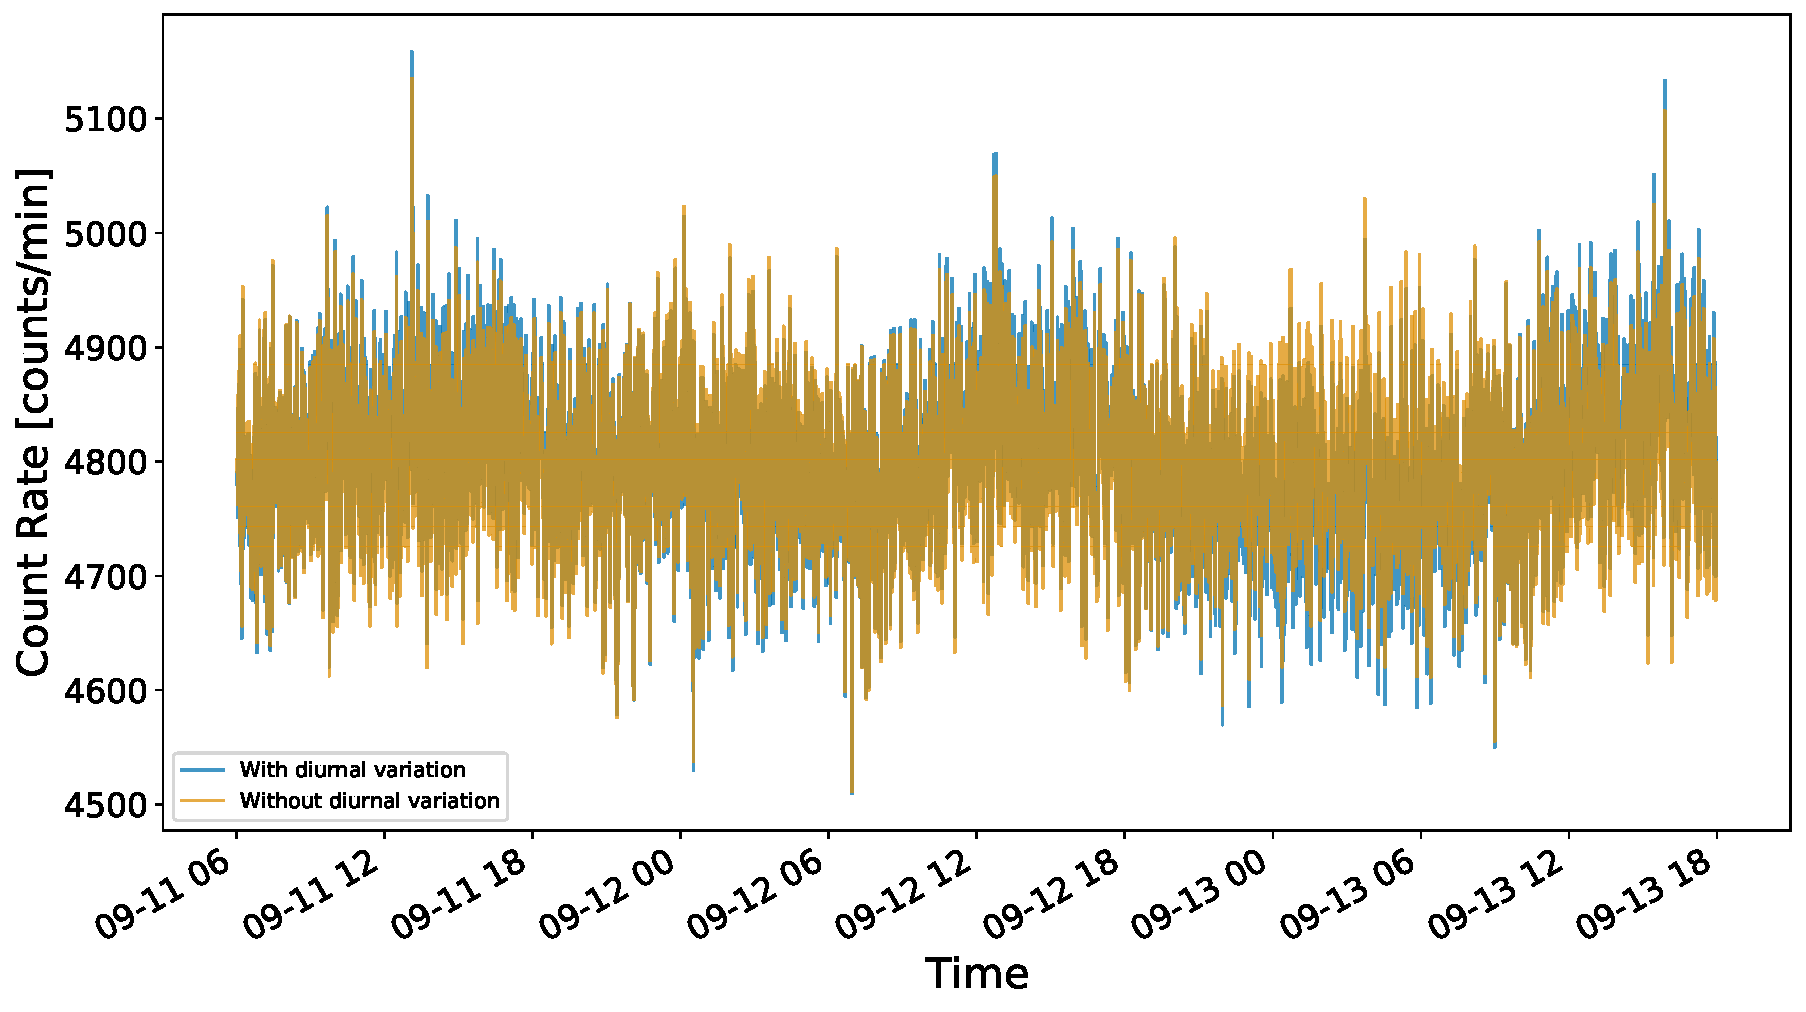
\includegraphics[width=\columnwidth]{many_day_diurnal_effect_timeseries.pdf}
	\caption{Time series of coincidences data, corrected for atmospheric pressure and displaying the diurnal variation with a peak at around midday.}
	\label{fig:corrected_coinciences}
\end{figure}


As the counts follow a Poisson distribution we sampled the data using the {\verb pymc3 } \gls{nuts} extension to a \gls{hmc} sampling algorithm \citep{salvatier_probabilistic_2016} with a Poisson distribution likelihood function. This allowed us to determine the mean count rate. Convergence was interrogated using the $\widehat{R}$ diagnostic factor using the criteria that chains did not converge if $\widehat{R} > 1.01$. 

%The distribution of the random coincidences is shown in Figure~\ref{fig:poisson_coinciences_dist}.
%
%
%\begin{figure}[ht!]
%	\centering
%	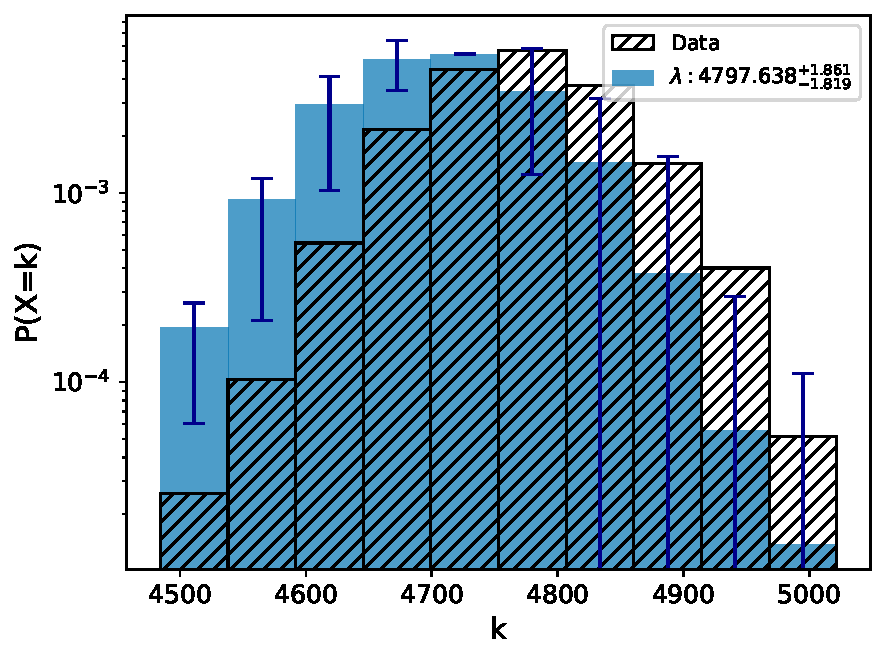
\includegraphics[width=0.9\columnwidth]{fitted_poisson.pdf}
%	\caption{Distribution of ... and Poisson distribution of the random coincidences, along with the median posterior fitted mean of the sample...}
%	\label{fig:poisson_coinciences_dist}
%\end{figure}


The median value of the posterior distribution for the mean value of the Poisson distribution of these coincidence data is $4797 \pm 2$~counts/min, where the uncertainties represent the $68 \%$ credible intervals either side of the median. We therefore have a count rate of $\sim 80 \, \upmu/\mathrm{s}$ in this stacked detector configuration. This is lower than the estimates predicted in the simulations in Chapter~\ref{chap:HiSPARC}, but is close to the predicted values for the non-vertical simulations, which represent a good approximation to the true muon flux at ground level. With a count rate of count rate of $\sim 80 \, \upmu/\mathrm{s}$, the Poisson noise is a rate of $\sim 9 \, \upmu/\mathrm{s}$, which represents $\sim 11 \%$ of the signal.


These observations have shown the full coincidences data, which are stored only locally. The data sent to the \gls{hisparc} servers are the reduced counts, which use the \gls{nim} gate signal to reduce the count rate by a factor of $\sim 100$. This data is also stored locally, but the data are acquired slightly differently. As discussed in Section~\ref{sec:HS14008_data_acqusition}, the reduced counts stored locally use the \gls{nim} counter to count the rate of the external trigger signal (i.e. coincidences between the \gls{nim} gate signal, and the coincidences between the two \glspl{pmt}). The \gls{hisparc} events data uses this trigger to read the events directly from the \glspl{pmt}. Due to the delays in the signal in the \gls{nim} create, one could reasonably have a concern that the two sources of data may differ. In Figure~\ref{fig:reduced_coincidences} we show a comparison between the reduced coincidences data stored locally and those recorded as events data in the \gls{hisparc} server.

%\begin{figure}[ht!]
%	\centering
%	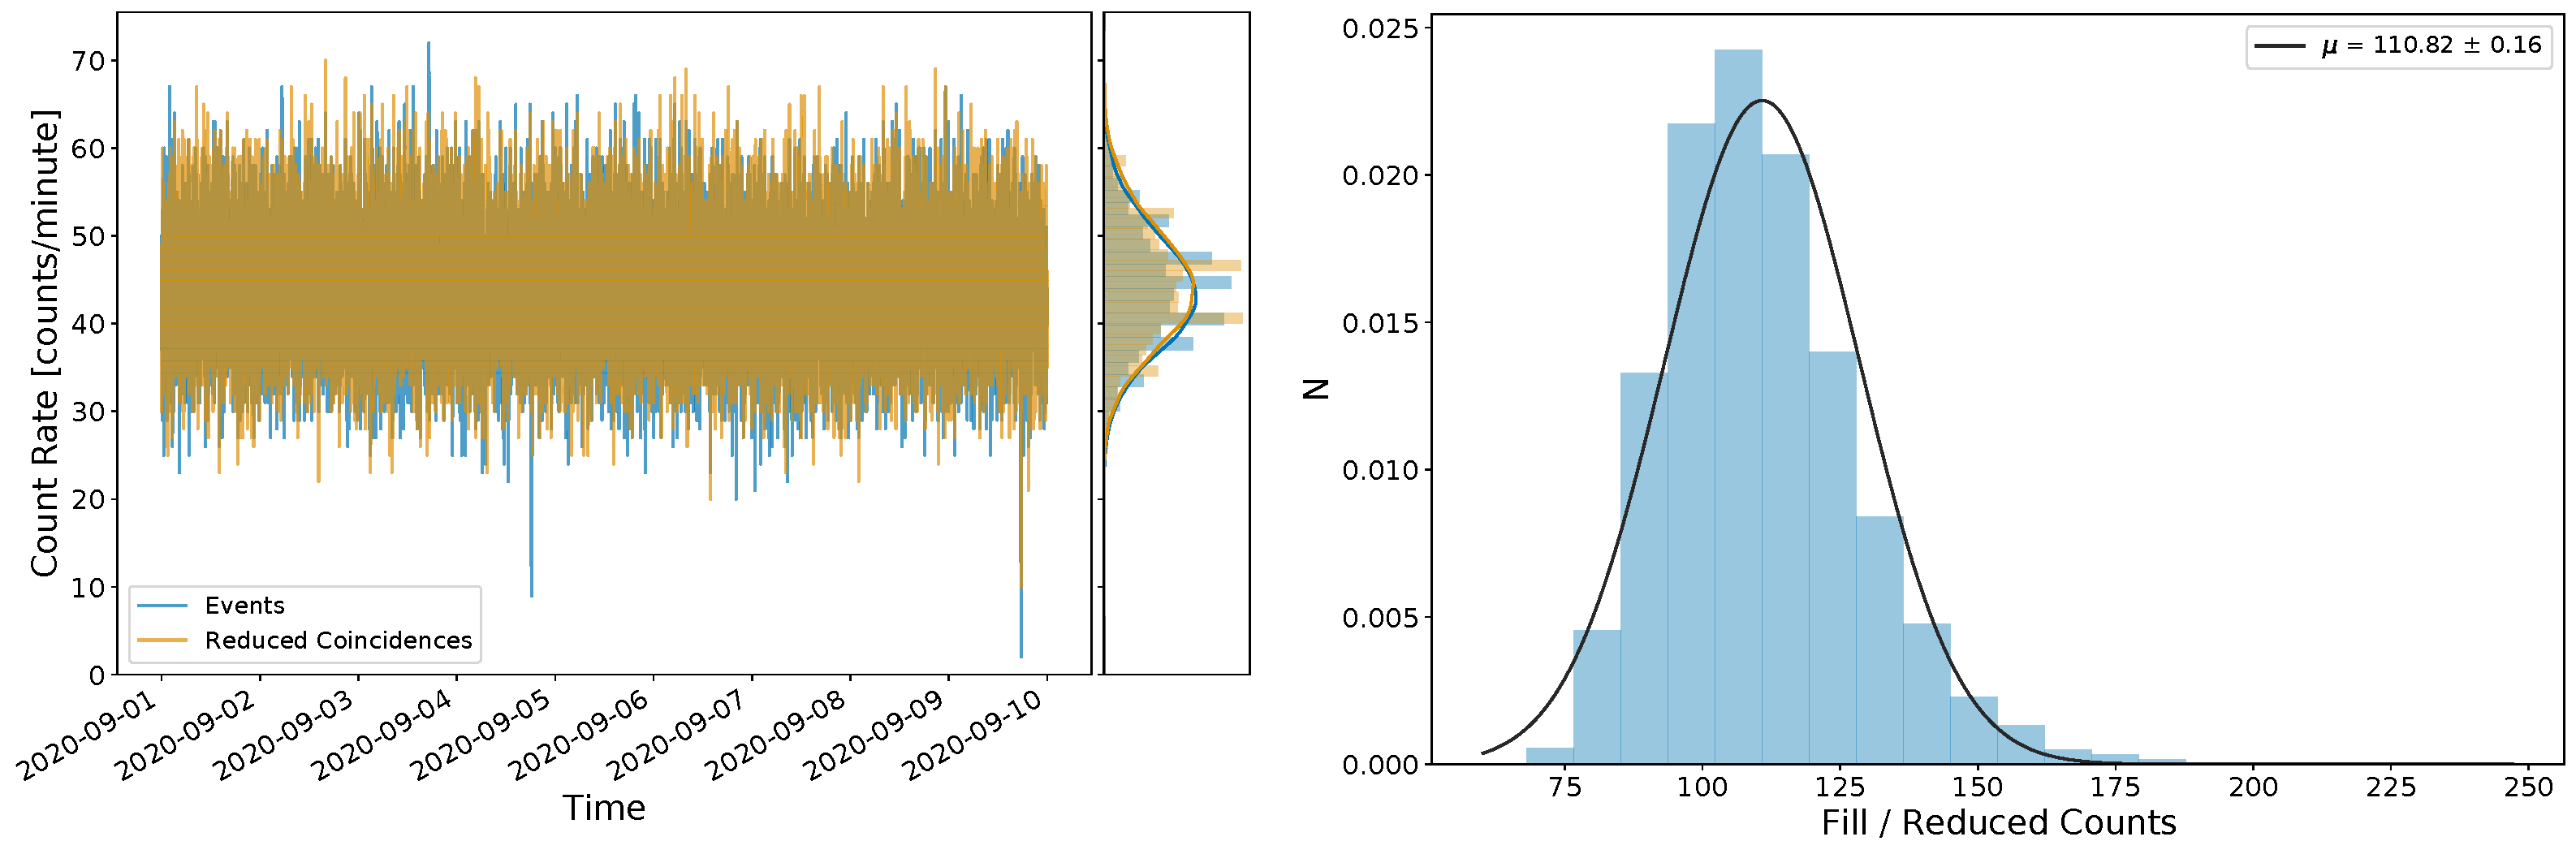
\includegraphics[width=\columnwidth]{reduced_coinc.pdf}
%	\caption{Comparison of the reduced coincidences stored locally and as events data in the HiSPARC server (left); }
%	\label{fig:reduced_coincidences}
%\end{figure}

\begin{figure}[ht!]
	\centering
	\subfloat[Timeseries of reduced coincidences]{
		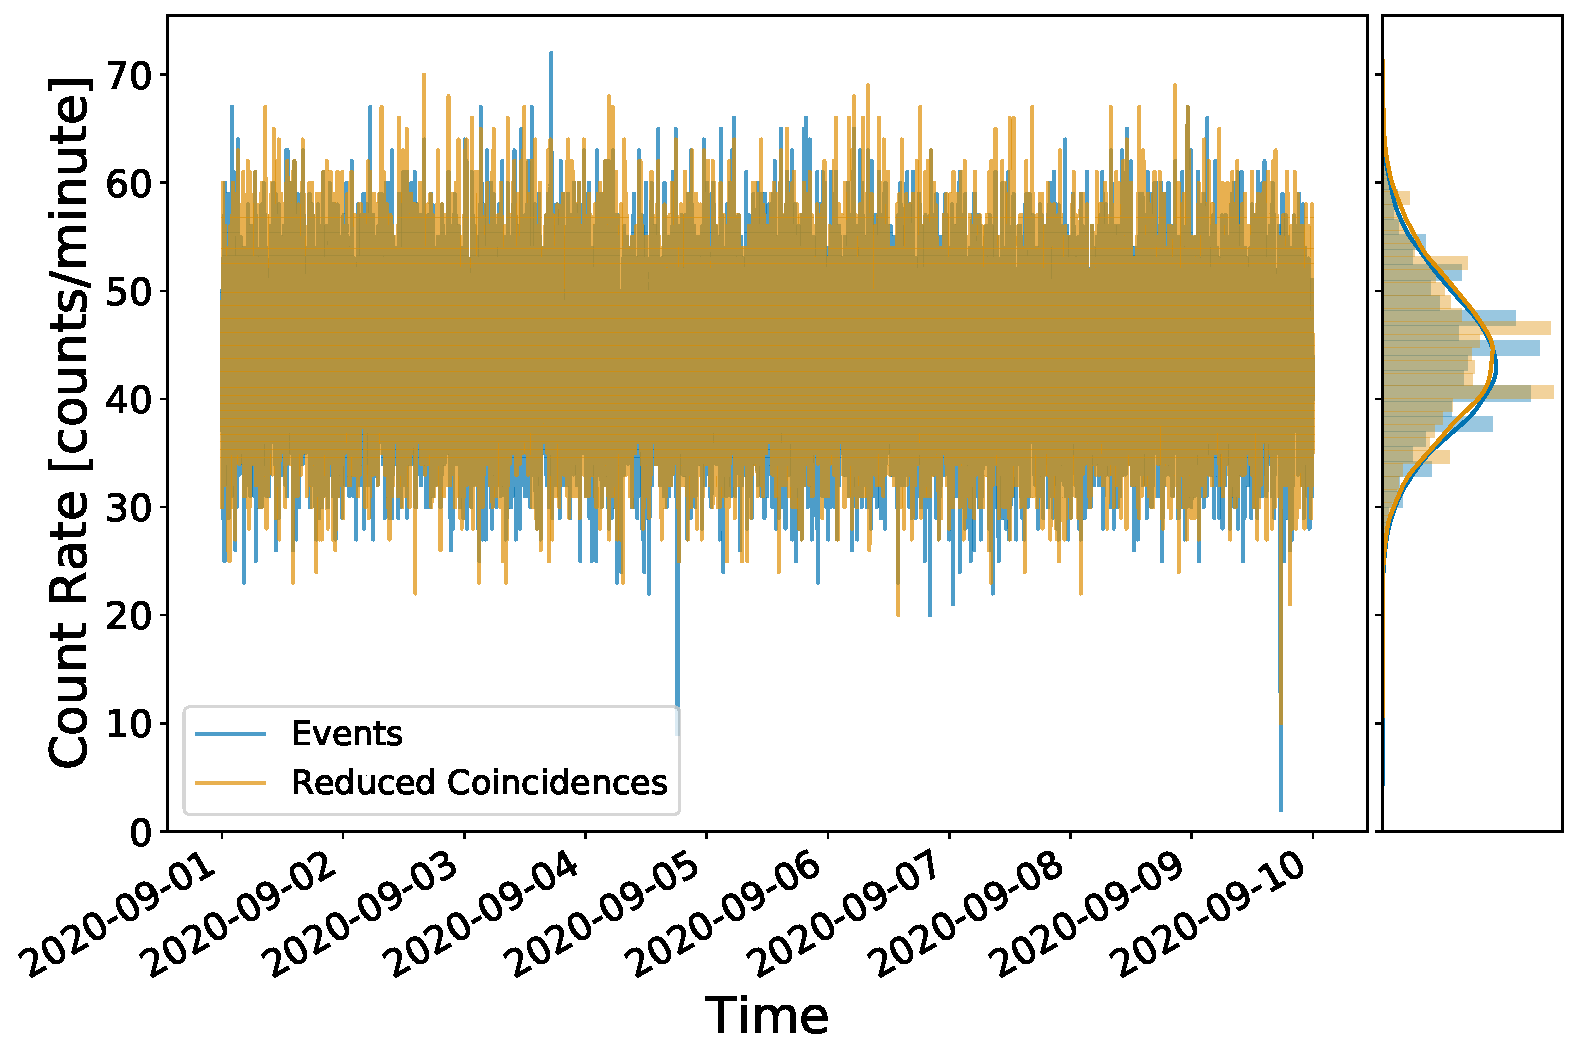
\includegraphics[width=0.52\columnwidth]{reduced_events_vs_coinc.pdf}
		\label{fig:rc1}}
	%\qquad
	\subfloat[Distribution of full-to-reduced coincicdences ratio]{
		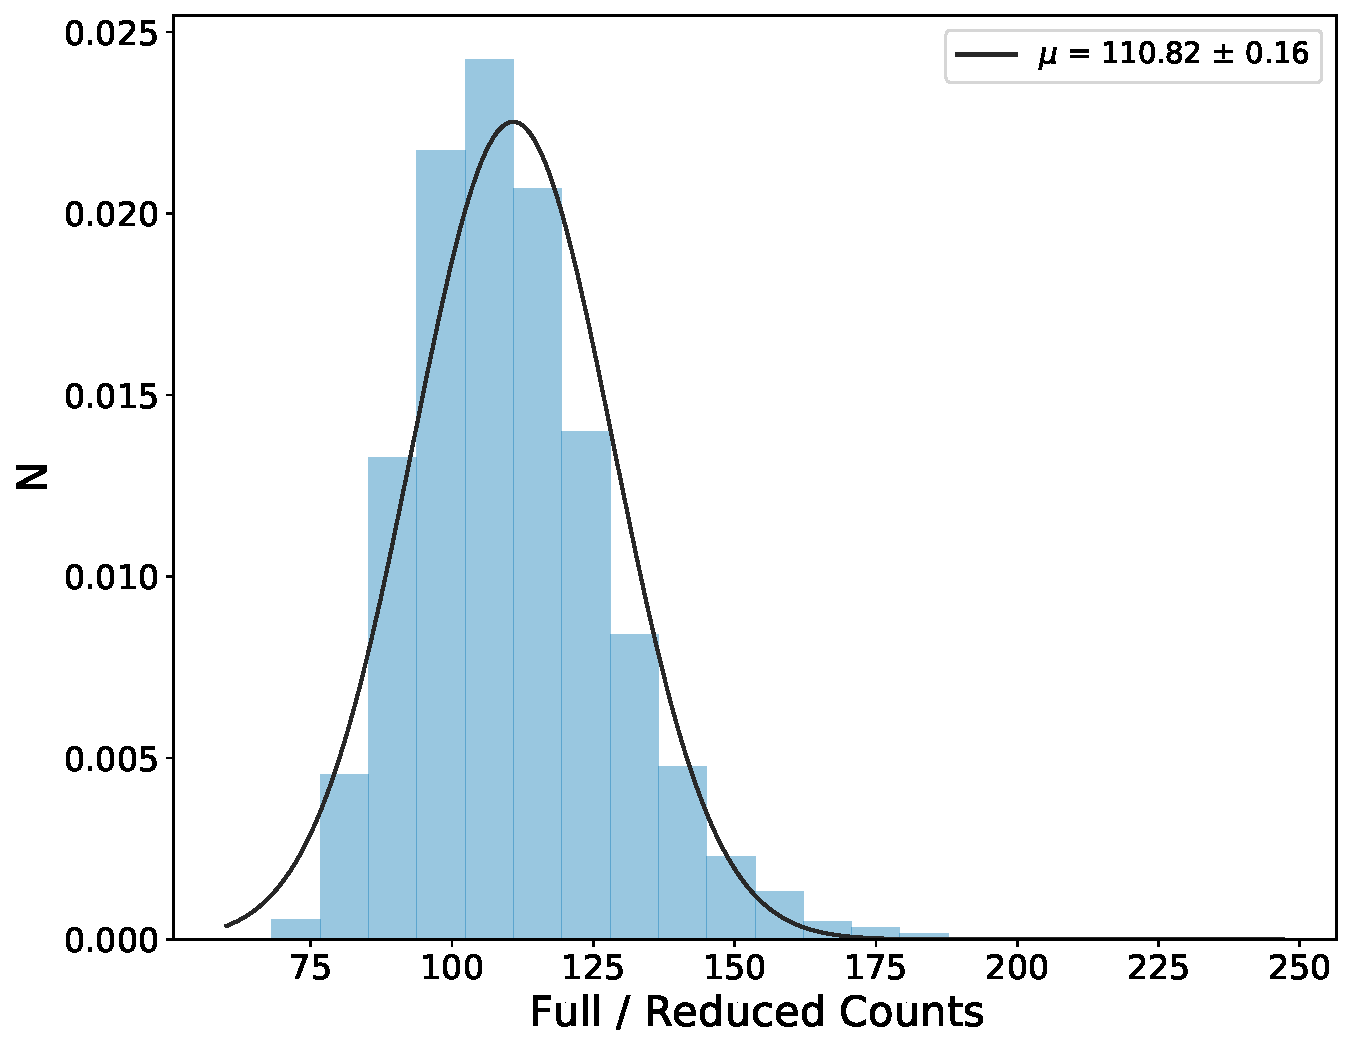
\includegraphics[width=0.44\columnwidth]{coinc_reduction_factor.pdf}
		\label{fig:rc2}} \\
	
	\caption{(a) Comparison of the reduced coincidences stored locally (orange) and as events data in the HiSPARC server (blue). (b) Distribution of the ratio of the full and reduced coincidence rates.}
	\label{fig:reduced_coincidences}
\end{figure}

The mean value of the Poisson distribution of these coincidence data is $\sim 44$~counts/min ($\sim 0.73 \, \upmu/\mathrm{s}$), which is a reduction by a factor of $\sim 110$ from the full coincidences data. We can see from Figure~\ref{fig:reduced_coincidences} that both the data stored locally (reduced coincidences) and the data sent to the \gls{hisparc} server (events) are in agreement, with only the realisation of the noise being different between the data. The \gls{hisparc} data acquisition software features a pre-trigger window (duration: $1 \, \upmu\mathrm{s}$), coincidence window (duration: $1.5 \, \upmu\mathrm{s}$), and a post-trigger window (duration: $3.5 \, \upmu\mathrm{s}$). The duration of these coincidence windows means that any delay on the order of $\sim 10$~ns is small, and does not effect the ability of the data acquisition software to record the data from the external trigger. This verifies that the locally stored reduced coincidences data and the events data stored in the \gls{hisparc} sever are measuring the same signal. With a count rate of count rate of $\sim 0.73 \, \upmu/\mathrm{s}$, the Poisson noise is on the same order of magnitude as the signal.


To understand the noise properties of this new configuration we investigated the random noise which is induced by random/spurious counts between both \glspl{pmt} and do not coincide with the passage of a muon. This was achieved by adding a delay in the signal between the two \glspl{pmt}, to ensure any coincident triggers were not due to true coincidences from the passage of a muon. By adding additional cables to the output from one \gls{pmt}, a delay of $\sim 120$~ns was added between the two signals. The \gls{fwhm} of a typical pulse from the \glspl{pmt} is $\sim$~25~ns, and the total duration from beginning-to-end is on the order of 100~ns \citep{van_dam_hisparc_2020}, therefore the $\sim 120$~ns delay was sufficient to remove true coincidences from the observations.

The delay was added between the two PMTs for around a week and the time series of the coincidences are shown in Figure~\ref{fig:random_coinciences}. We can see that the noise is nominally $\sim 1$~count/minute.

\begin{figure}[ht!]
	\centering
	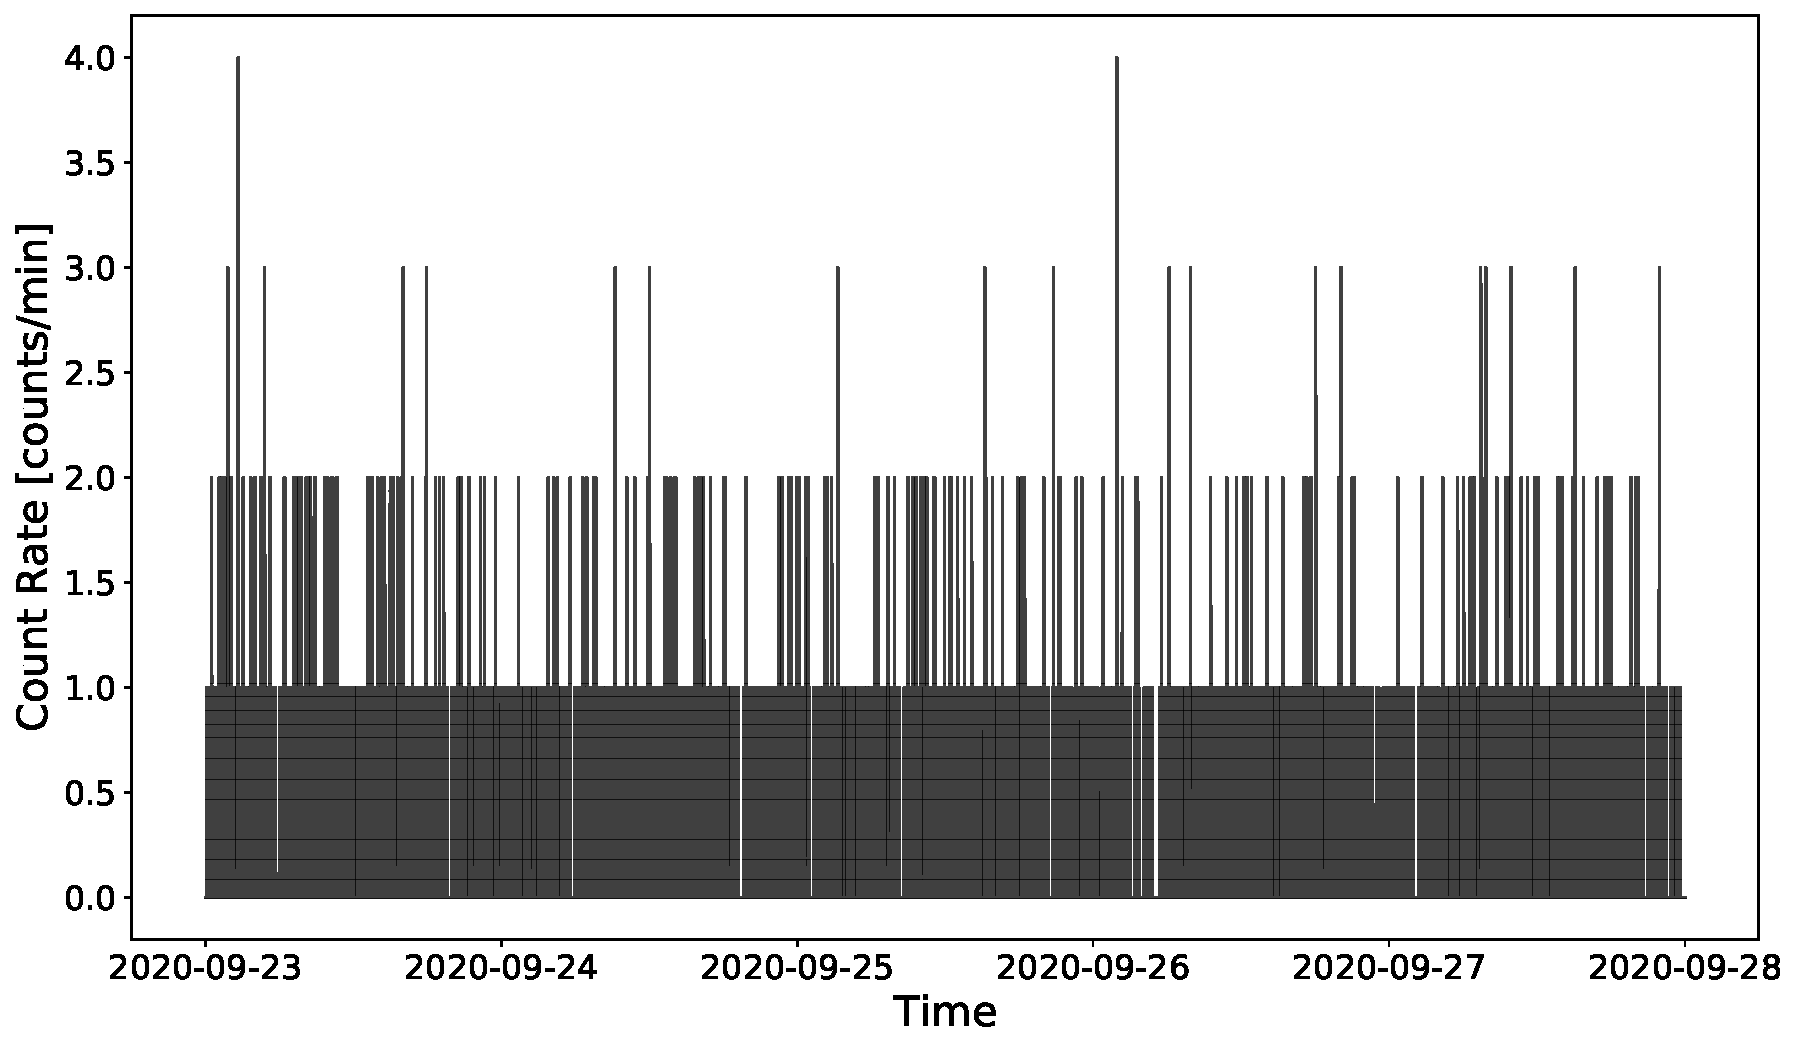
\includegraphics[width=\columnwidth]{random_noise_timeseries.pdf}
	\caption{Time series of random coincidences data...}
	\label{fig:random_coinciences}
\end{figure}

We know the noise must follow a Poisson distribution, therefore we aimed to quantify the mean value of the noise. The noise was sampled to determine the mean of the Poisson distribution using the {\verb pymc3 } \gls{nuts} extension to a \gls{hmc} sampling algorithm \citep{salvatier_probabilistic_2016}. Convergence was interrogated using the $\widehat{R}$ diagnostic factor using the criteria that chains did not converge if $\widehat{R} > 1.01$. The distribution of the random coincidences is shown in Figure~\ref{fig:random_coinciences_dist}

\begin{figure}[ht!]
	\centering
	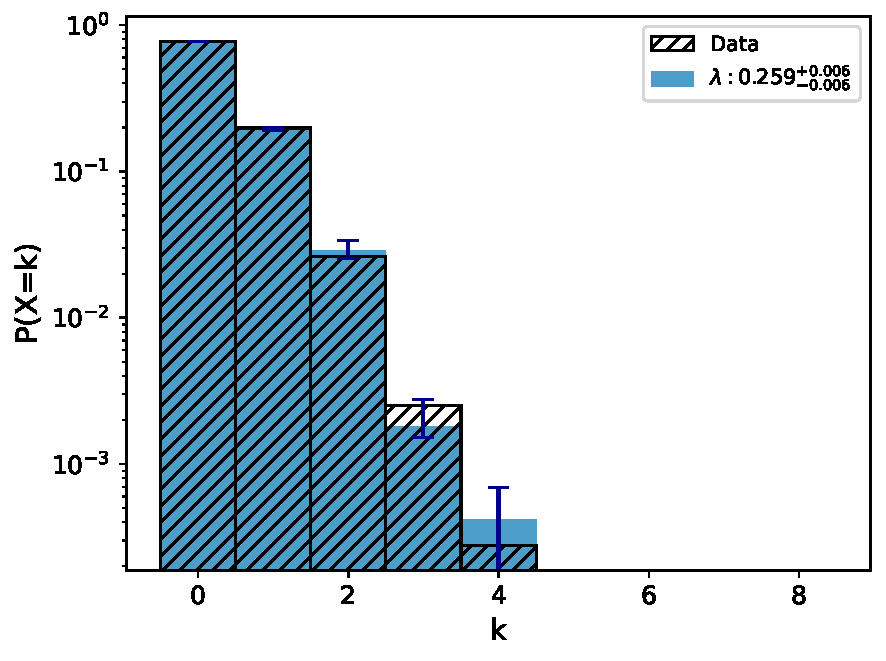
\includegraphics[width=0.9\columnwidth]{random_noise_fitted_poisson.pdf}
	\caption{Distribution of random coincidences data... and Poisson distribution of the random coincidences, along with the median posterior fitted mean of the sample...}
	\label{fig:random_coinciences_dist}
\end{figure}

The median value of the posterior distribution for the mean value of the Poisson distribution of random coincidence is $0.259 \pm 0.006$~counts/min, where the uncertainties represent the $68 \%$ credible intervals either side of the median. This represents a small noise; under this Poisson likelihood function the probability of no noise is $\sim 77 \%$, 1~count/minute is $\sim 20 \%$, and over 2~counts/minute is $< 3 \%$.

It is also important to note that in Figure~\ref{fig:random_coinciences}, there is no diurnal signal in the random noise. This shows that as the \gls{pmt} thermal noise increases around midday, which we see manifesting in the singles data, the increased thermal noise does not manifest in the spurious coincidences between both \glspl{pmt}. This is important as it highlights that in this stacked detector configuration we have maximised our ability to observe single muons whilst reducing the effects of diurnal, thermally induced noise.



%%%%%%%%%%%%%%%%%%%%%%%%%%%%%%%%%%%%%%%%%%%%%%%%%%%%%%%%%%%%%%%%%%%%%
%%%%%%%%%%%%%%%%%%%%%%%%%%%%%%%%%%%%%%%%%%%%%%%%%%%%%%%%%%%%%%%%%%%%%
\subsection{Comparison with Neutron Monitors}\label{sec:HS_14008_vs_Kiel}

It is useful to compare the data from this new \gls{hisparc} station to an existing \gls{nm} detector, as this can highlight whether any confirmed space weather events using the \gls{gnmn} have been observed with this new configuration. There were no space weather events from the beginning of \gls{hisparc} station 14008 operation to the time of writing; however, we still show a comparison to a nearby \gls{nm} station.

The Kiel \gls{nm} station, in Germany, used in Chapter~\ref{chap:HiSPARC} had suffered difficulties with data consistency during this epoch, therefore another station was used for the analysis here. We chose to analyse the \gls{nm} count rate at, Dourbes, which is located in Belgium and is the nearest \gls{nm} to the \gls{hisparc} network, at $\sim 525$~km away from stations 14008 in Birmingham. The properties of the Dourbes station are: $R_C$=3.18~GV, Altitude=225~m, Latitude=$50.10^{\circ}$N, Longitude=$4.59^{\circ}$E \citep{nmdb_nmdb_nodate}. In Figure~\ref{fig:14008_vs_DRBS}, a comparison is shown between the \gls{hisparc} data and the Dourbes \gls{nm} station during November 2020.

\begin{figure}[ht!]
	\centering
	\subfloat[HS 14008 vs Dourbes (offset)]{
		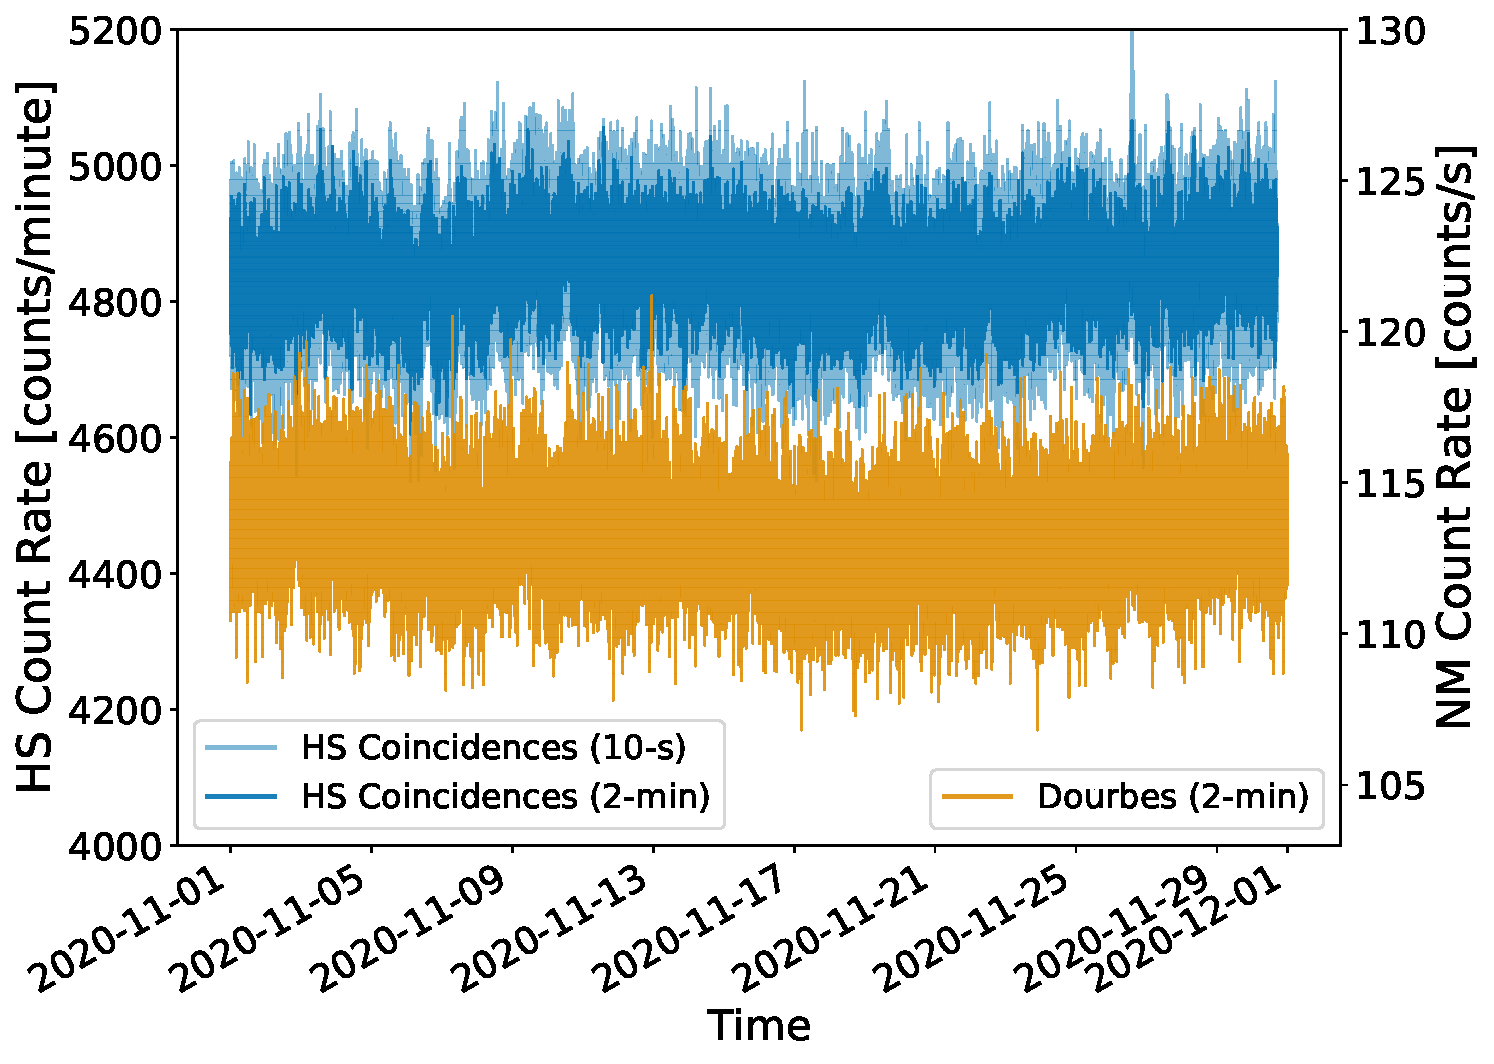
\includegraphics[width=0.48\columnwidth]{HS14008_vs_DRBS.pdf}
		\label{fig:14008vsDRBS_1}}
	%\qquad
	\subfloat[HS 14008 vs Dourbes (overlay)]{
		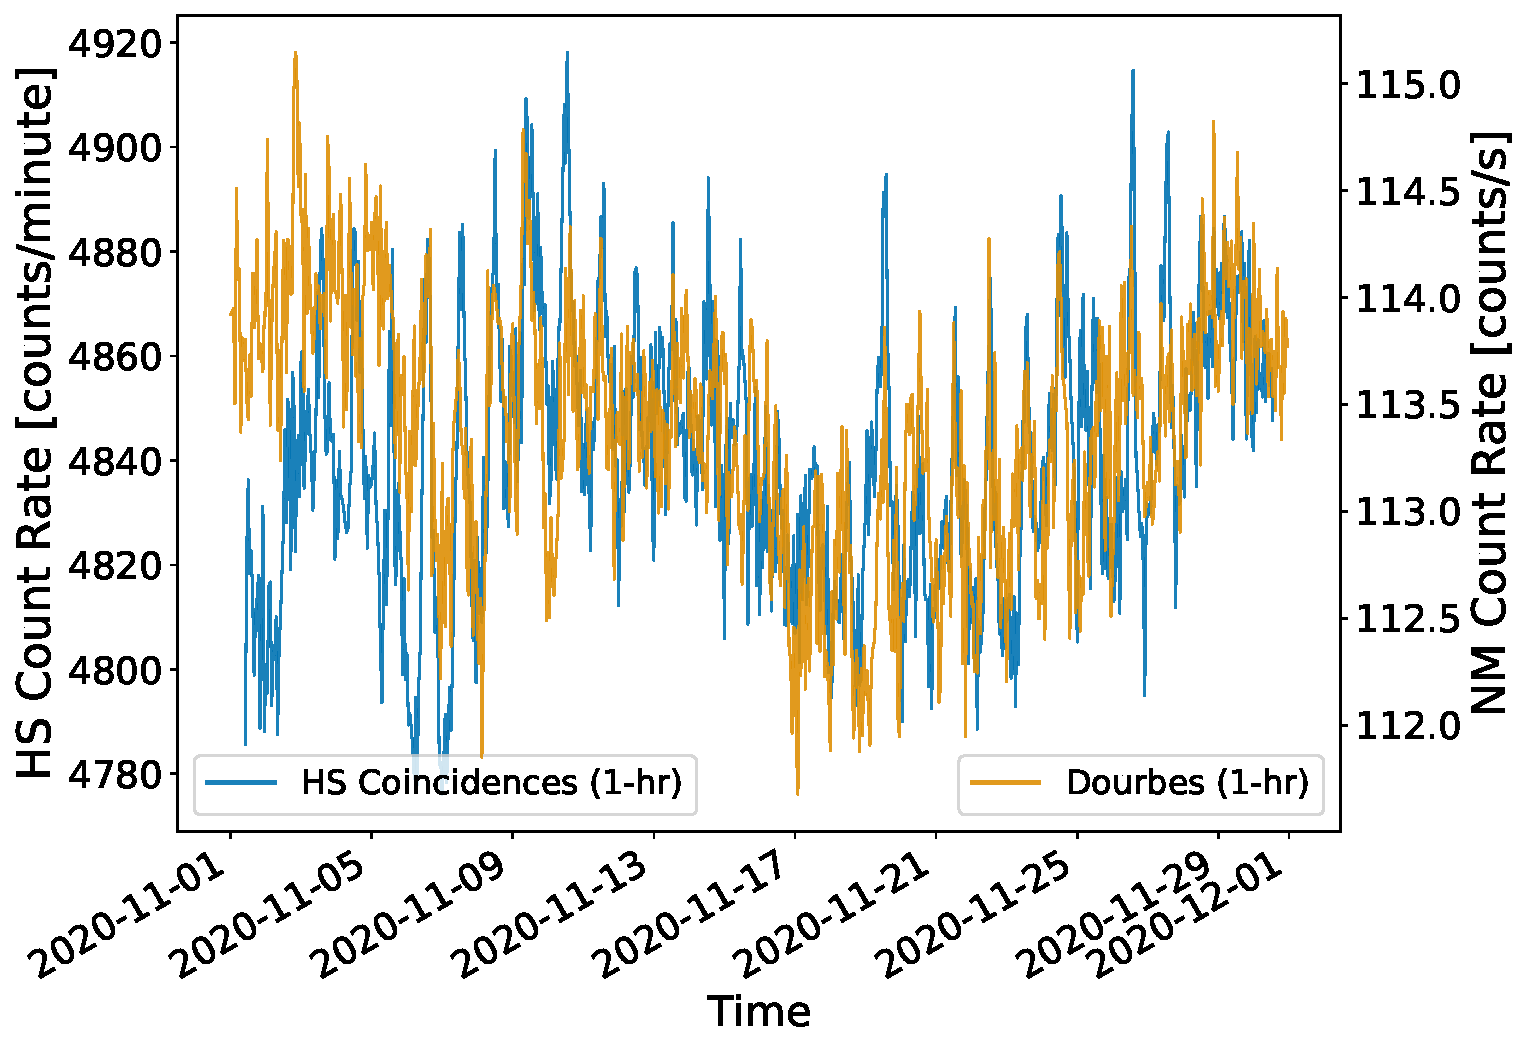
\includegraphics[width=0.48\columnwidth]{HS14008_vs_DRBS_overlay.pdf}
		\label{fig:14008vsDRBS_2}} \\

	
	\caption{...}
	\label{fig:14008_vs_DRBS}
\end{figure}


The plots in Figure~\ref{fig:14008_vs_DRBS} show a good visual agreement between the two detectors. Despite a good visual agreement, the Pearson correlation coefficient is $\rho \sim 0.08$, highlighting that there is no correlation between the two stations, at the 2-minute level. When resampling the data to 1-hour and 1-day the correlation increases to $\rho \sim 0.38$ and $\rho \sim 0.41$, respectively. This shows a weak, low frequency correlation between the two stations. This weak correlation shows the two stations monitor approximately the same background \gls{cr} signal, which is relatively flat as the solar activity is low, therefore contributions from \glspl{scr} is low. At the 2-minute level, the near--zero correlation demonstrates that the variations in the two signals are dominated by noise and there is no covarying signal.

This comparative analysis should be continually monitored, and particularly used as a reference when any space weather events are recorded with the \gls{gnmn}. As they are the closest stations to the \gls{hisparc} 14008 detector in Birmingham, it is useful to continue using the Dourbes \gls{nm} station, but also to incorporate the Kiel \gls{nm} station, where issues with data quality are resolved. Near the maximum of Solar Cycle 25, expected 2023 -- 2026 and likely to arrive in 2025 \citep{mcintosh_overlapping_2020, pesnell_lessons_2020}, we would expect the correlation to grow as the number of \glspl{sep} increases. It is therefore important that this configuration of \gls{hisparc} detector is maintained until at least 2026, to ensure a complete study is performed.


%%%%%%%%%%%%%%%%%%%%%%%%%%%%%%%%%%%%%%%%%%%%%%%%%%%%%%%%%%%%%%%%%%%%%
\subsection{Single Station Space Weather Uses}\label{sec:HS_14008_single_sims}

Simulations of artificial data were performed to determine the magnitude of \glspl{gle} that may be observed in this new detector configuration, as described in Section~\ref{sec:HS_14008_method_obs}. As we have shown, the \gls{hisparc} 14008 station has a background, mean count rate, $\lambda \sim 80 \, \upmu/\mathrm{s}$, and a noise of $\sigma \sim 0.26 \, \upmu/\mathrm{s}$. These were used as inputs to the simulations, where \glspl{gle} were simulated with amplitudes of: $1.0\%$, $1.5\%$, $2.0\%$, $2.5\%$, $3.0\%$, $3.5\%$, $4.0\%$, $4.5\%$, $5.0\%$, $7.5\%$, and $10.0\%$. The start times, rise and decay times were all randomly sampled and the statistics tests performed on the resultant data.

Running several iterations, it was possible to analyse the statistics of the resultant data for each amplitude of \gls{gle} and compare it to the background signal of the detector, without a \gls{gle} signal. An example of the statistical tests on a single iteration is shown in Figure~\ref{fig:simulated_data_stats}, for a $10 \%$ \gls{gle} magnitude and a table showing the average number of statistically significant measurements for a simulation without an injected \gls{gle} is shown in Table~\ref{tab:HS_14008_sims_zeros}.


\begin{figure}[ht!]
	\centering
	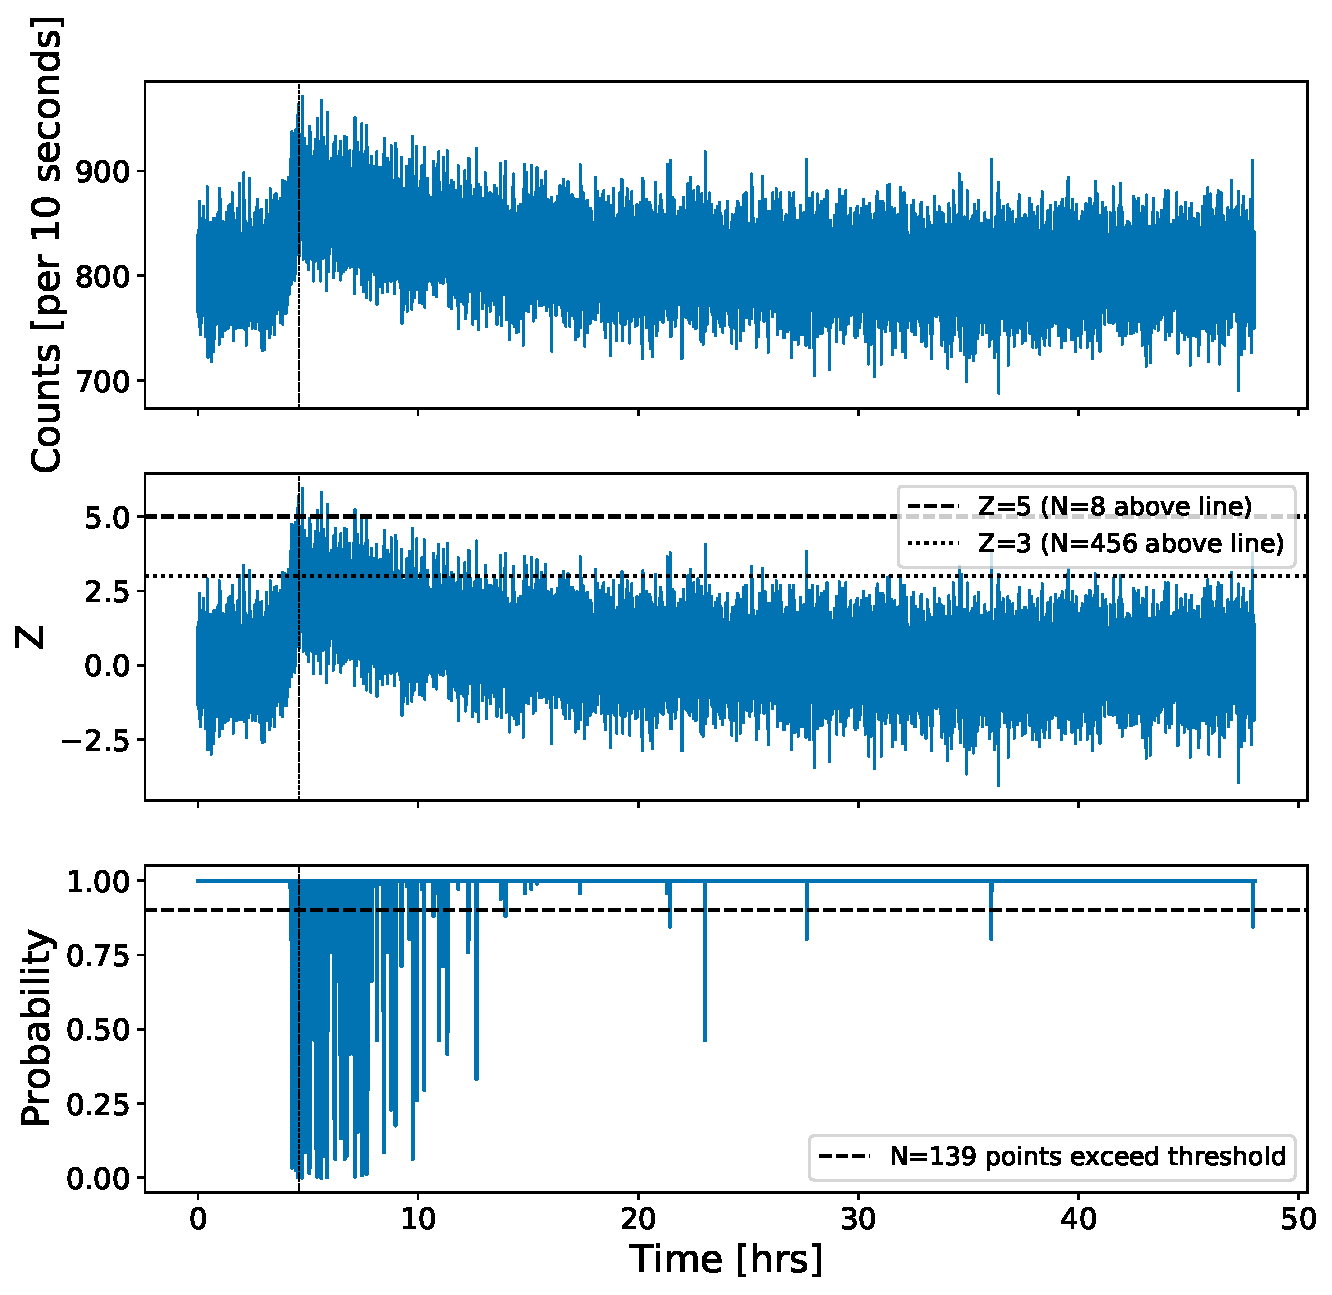
\includegraphics[width=0.9\columnwidth]{simulated_data_stats.pdf}
	\caption{Single realisation of a simulation with a $10\%$ \gls{gle} magnitude. Top panel shows the raw, artificial data from the simulation, with a 10-second cadence. Middle panel shows the number of measurements exceeding the $Z=3$ and $Z=5$ thresholds. The $Z=3$ and $Z=5$ thresholds are depicted as dotted and dashed lines, respectively. Bottom panel shows the number of points exceeding the $p = 10 \%$ threshold in the binomial test, where a low probability value indicates a high statistical significance.}
	\label{fig:simulated_data_stats}
\end{figure}


\begin{table}[ht!]
	\begin{center}
		\caption{... with no injected GLEs ...}
		\label{tab:HS_14008_sims_zeros}
		\begin{tabular}{c c c c}
			\hline 
			{} & \multicolumn{3}{c}{\bf No. significant measurements} \\ 
			{\bf Data cadence} & {\bf Binomial} & {\bf $\mathbf{Z=3}$} & {\bf $\mathbf{Z=5}$}  \\ 
			\hline 
			10-second & $2^{+2}_{-1}$ & $27^{+6}_{-5}$ & $0 \pm 0$ \\ 
			1-minute & $2^{+1}_{-2}$ & $4 \pm 2$ & $0 \pm 0$ \\ 
			5-minute & $1 \pm 1$ & $1 \pm 1$ & $0 \pm 0$ \\ 
			\hline 
		\end{tabular} 
	\end{center}
\end{table}

The results in Table~\ref{tab:HS_14008_sims_zeros} provides the expected number of statistically significant fluctuations in the noise for each test method applied to the raw and resampled data. For a particular two day observation, we can say that any epoch with statistically significant peaks in excess of these values can be treated as statistically significant, and it is likely that there was a space weather event. We expect that any measurements which exceed the $Z=5$ should clearly be treated as a significant event, as within two days of artificial data, we observed no random fluctuations in the noise exceeding this level. In addition, we see that there is a large difference in the number of measurements exceeding the $Z=3$ threshold between the raw, 10-s data to 5-minute averaged data. We can be confident of there being a true event if the number of significant measurements exceeds $\sim 33$, $\sim 6$, and $\sim 2$, for the raw data, 1-minute averaged data, and 5-minute averaged data, respectively. Finally, in the case of the binomial test, the average number of statistically significant fluctuations in the noise exceeding the $10 \%$ threshold is in the range $\sim 2-4$. We expect that the binomial method is a good measure of the existence of a true event, due to the consistency of the sensitivity, regardless of averaging over the data. 

In the data, we can use the number of statistically significant measurements to warn whether there exists a possible event in the data, and closer inspection of the statistics tests can verify of exclude the existence of a true event. For example, in Figure~\ref{fig:simulated_data_stats}, there are 139 points exceeding the $10 \%$ binomial limit, and 456 and 8 point above the $Z=3$ and $Z=5$ limits, respectively. This indicates the existence of an event in the data. On closer inspection it is clear from the grouping of the number of points exceeding each of the thresholds where the event occurred.

For each \gls{gle} magnitude we ran 1000 iterations of the simulations and were able to average over the number of statistically significant events observed for a given \gls{gle} magnitude. This was done for the raw, 10-s cadence data and further simulations were performed for 1-minute averaging and 5-minute averaging, independently.

To summarise the results of all the simulations, Figure~\ref{fig:single_HS14008_sims} shows the average number of cadences with statistically significant measurements against the simulated \gls{gle} magnitude for the 10-s cadence observations, 1-minute and 5-minute averages. The horizontal, dashed lines shows the median number of random significant observations, i.e. without an injected \gls{gle}, and the horizontal, dotted lines represent the $68 \%$ credible intervals either side of the median. Each point shows the median number of statistically significant observations for different \gls{gle} magnitudes, with error bars representing the $68 \%$ credible intervals either side of the median.


\begin{figure}[!htbp!]
	\centering
	\subfloat[10-s cadence simulation]{
		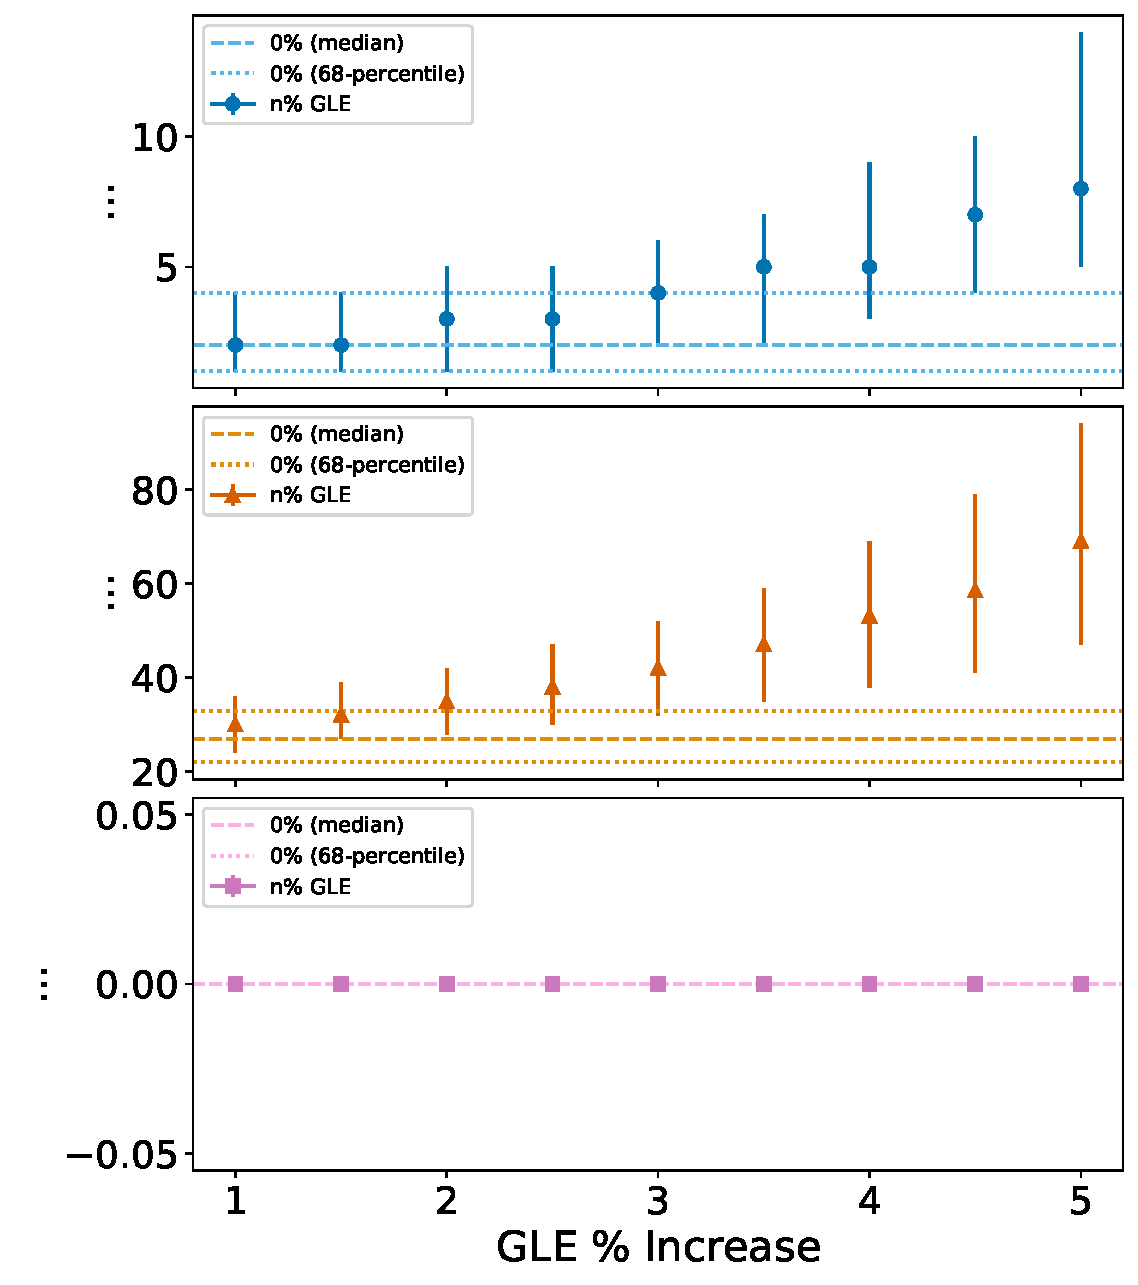
\includegraphics[width=0.48\columnwidth]{HS_14008_sims_plot_0rebin.pdf}
		\label{fig:single_sims_0min_rebin}}
	%\qquad
	\subfloat[1-minute averaging]{
		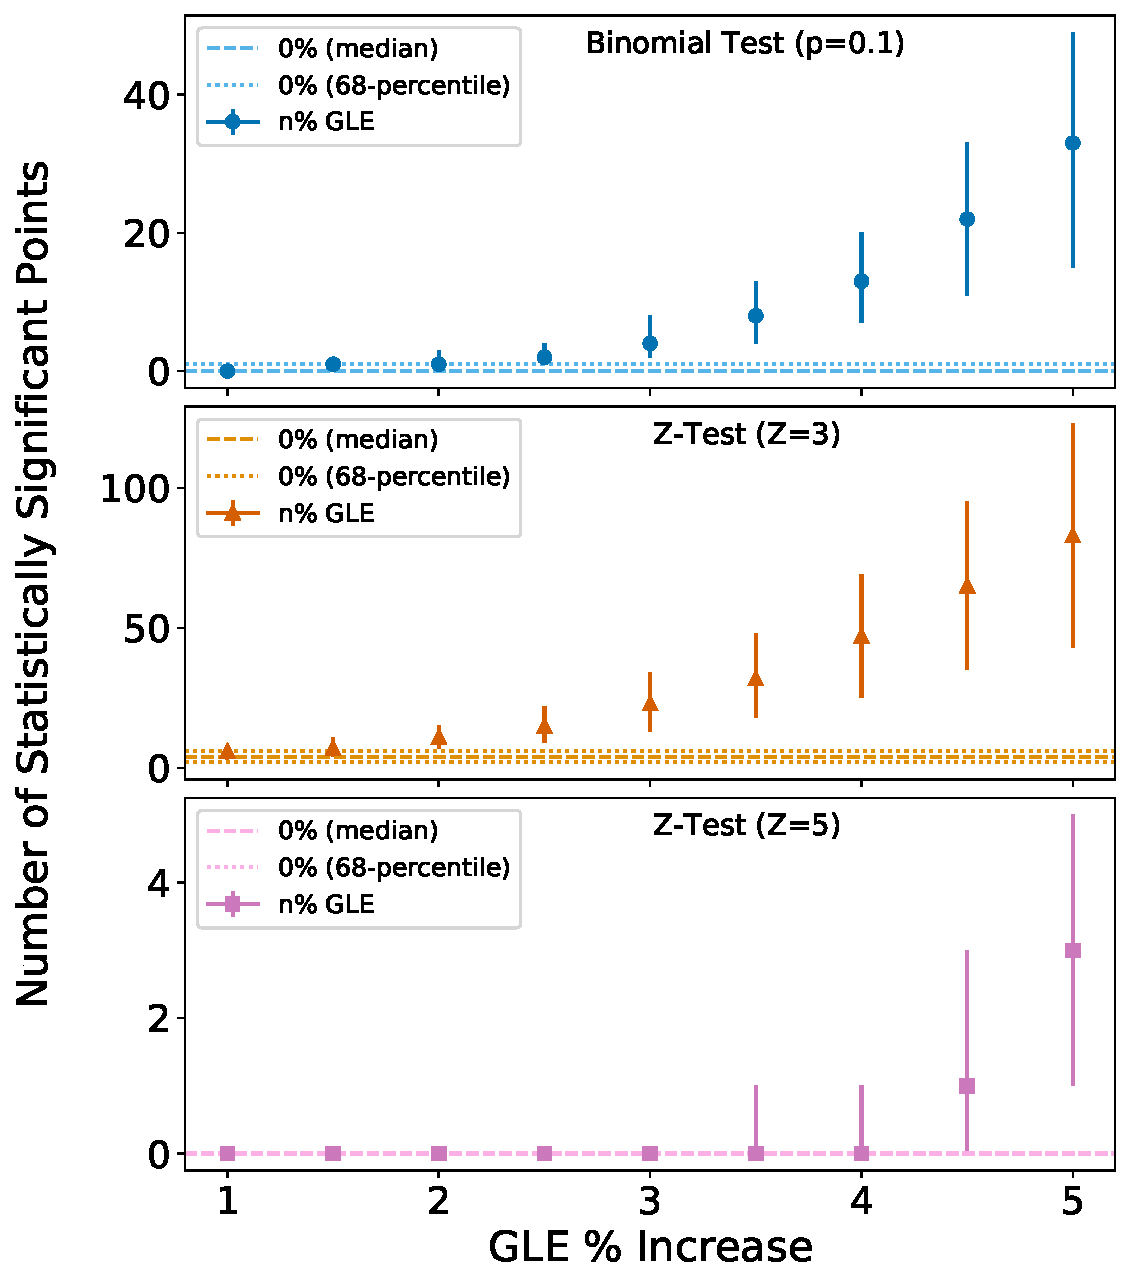
\includegraphics[width=0.48\columnwidth]{HS_14008_sims_plot_1rebin.pdf}
		\label{fig:single_sims_1min_rebin}} \\
	%\qquad
	\subfloat[5-minute averaging]{
		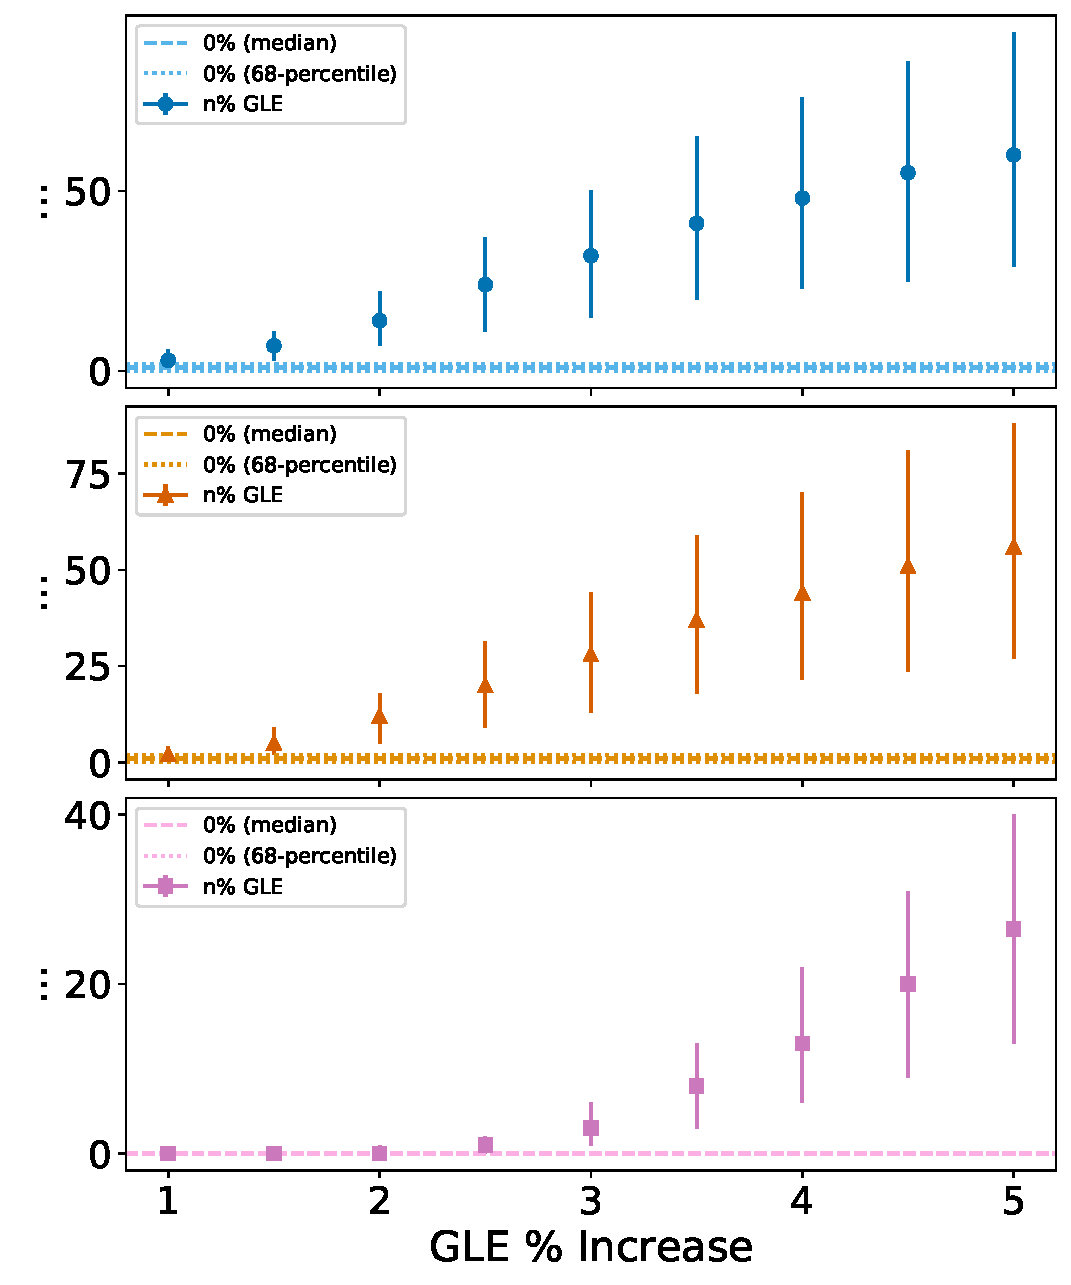
\includegraphics[width=0.48\columnwidth]{HS_14008_sims_plot_5rebin.pdf}
		\label{fig:single_sims_5min_rebin}} \\
	
	\caption{Summary plots showing the number of statistically significant measurements using the binomial- and Z-tests on the simulations of artificial data with varying magnitudes of GLEs injected. (a) shows the results for the 10-s cadence data; (b) 1-minute averaged data; (c) 5-minute averaged data. In each plot, the top panel shows the number of significant points exceeding the binomial $p = 10 \%$ threshold, the middle panel shows the number of points exceeding the Z=3 threshold, and the bottom panel shows the number of points exceeding the Z=5 threshold. The dashed, horizontal lines show the median values of the tests without an injected GLE, and the horizontal, dotted lines represent the $68 \%$ credible intervals either side of the median. For each simulated GLE magnitude the point represents the median values and the error bars represent the $68 \%$ credible intervals either side of the median.}
	\label{fig:single_HS14008_sims}
\end{figure}

We see from Figure~\ref{fig:single_HS14008_sims} that in the case where no averaging of data is performed, using the $Z=3$ significance level, we expect to be able to differentiate the increase in the number of significant measurements for a \gls{gle} with magnitude of $> 3.0 - 3.5 \%$. Or using the binomial measure of significance, we expect to be able to differentiate the increase in the number of significant measurements for a \gls{gle} with magnitude of $> 4.5 - 5.0 \%$. To be able to see the results clearly, we only show the results for \gls{gle} magnitudes of up to $5\%$, and in Figure~\ref{fig:single_sims_0min_rebin}, we see using the $Z=5$ significance level, there are no significant observations for magnitudes $\leq 5\%$. In the full analysis, we investigated up to $10\%$, and determined that at the $Z=5$ significance level we can differentiate the increase in the number of significant events for \gls{gle} magnitude of $\geq 7.5\%$.

When averaging the data over 1-minute and 5-minute intervals, the detectable \gls{gle} magnitude at the $Z=3$ significance level drops to $2.0 - 2.5 \%$ and $\sim 1.5 \%$, respectively. Similarly, at the $Z=5$ significance level this drops to $4.5\%$ and $2.5 - 3.0 \%$, respectively. Finally, using the binomial measure of significance at the $p = 10 \%$ level, we expect to be able to differentiate the increase in the number of significant measurements for a \gls{gle} with magnitude of $2.0 - 2.5 \%$ and $\sim 1.0 - 1.5 \%$, respectively.

This shows that through averaging the data, we expect, with a single detector, that we should be able to detect a \gls{gle} which induces an increase in the muon count rate on the order of $1 - 2 \%$. Weighing the benefits of the increased sensitivity against the timescales observable, we recommend making use of the 1-minute averaged data rather than 5-minutes, as the durations of some space weather events can be short-lived, which makes it advantageous to not to average over an ephemeral signal.

Overall, based on the values predicted in Section~\ref{sec:MAIRE_flux}, we believe that it would have been possible to observe the increase in the muon count rate due to \gls{gle} 42, 43, and 45 with this new configuration. We have shown with the raw data we should be able to differentiate a \gls{gle} with magnitude $> 3\%$ (i.e. \gls{gle} 42) and when averaging the data into 5-minute bins, we expect to be able to observe \glspl{gle} with magnitudes $> 1.5 \%$  (i.e. \gls{gle} 43 and 45). 


%%%%%%%%%%%%%%%%%%%%%%%%%%%%%%%%%%%%%%%%%%%%%%%%%%%%%%%%%%%%%%%%%%%%%
\subsection{Multiple Station Space Weather Uses}\label{sec:HS_14008_multi_sims}


Many ground-based \gls{cr} detectors typically exist as part of a network, which work together to increase their combined sensitivity. With an increasing number of stations in a network, observing the same events, the combined sensitivity increases by a factor of $\sqrt{N}$, where $N$ is the number of stations in the network, due to the reduction in the Gaussian noise. However, it is also possible to use other methods to increase the sensitivity of the network and claim observations.

In this section we again use simulations of artificial data (see Appendix~\ref{app:GLE_sims} for details) to determine the magnitude of \glspl{gle} that may be observed with a network of detectors using this configuration. On overarching assumption in this multi-station analysis is that the detectors are all geographically close, such that the delay in the induced signals are minimal. This is for instance, assuming that we upgrade the \gls{hisparc} stations closest to the University of Birmingham. There are another five operational stations in Birmingham which are located within a radius of $<6$~km from this new configuration, and a sixth station within a radius of $\sim 15$~km from University of Birmingham; however, with the exception of the existing University of Birmingham station 14001, which is a 4-detector station, each of the stations in the Birmingham node is a 2-detector station. This means that there are in total an additional 14 individual detectors in the Birmingham node.



\begin{table}[ht!]
	\begin{center}
		\caption{... with no injected GLEs ...}
		\label{tab:HS_14008_multi_sims_zeros}
		\begin{tabular}{c c c c}
			\hline 
			{} & \multicolumn{3}{c}{\bf No. significant measurements} \\ 
			{\bf No. stations} & {\bf Binomial} & {\bf $\mathbf{Z=3}$} & {\bf $\mathbf{Z=5}$}  \\ 
			\hline 
			1 & $ 2^{+2}_{-1} $ & $ 27^{+6}_{-5} $ & $ 0 \pm 0 $ \\ 
			2 & $ 2^{+3}_{-1} $ & $ 26^{+22}_{-14} $ & $ 0 \pm 0 $ \\ 
			5 & $ 2^{+4}_{-2} $ & $ 25^{+23}_{-15} $ & $ 0 \pm 0 $ \\ 
			10 & $ 2^{+3}_{-2} $ & $ 25^{+32}_{-16} $ & $ 0 \pm 0 $ \\ 
			\hline 
		\end{tabular} 
	\end{center}
\end{table}



\begin{figure}[!htbp!]
	\centering
	\subfloat[1 station]{
		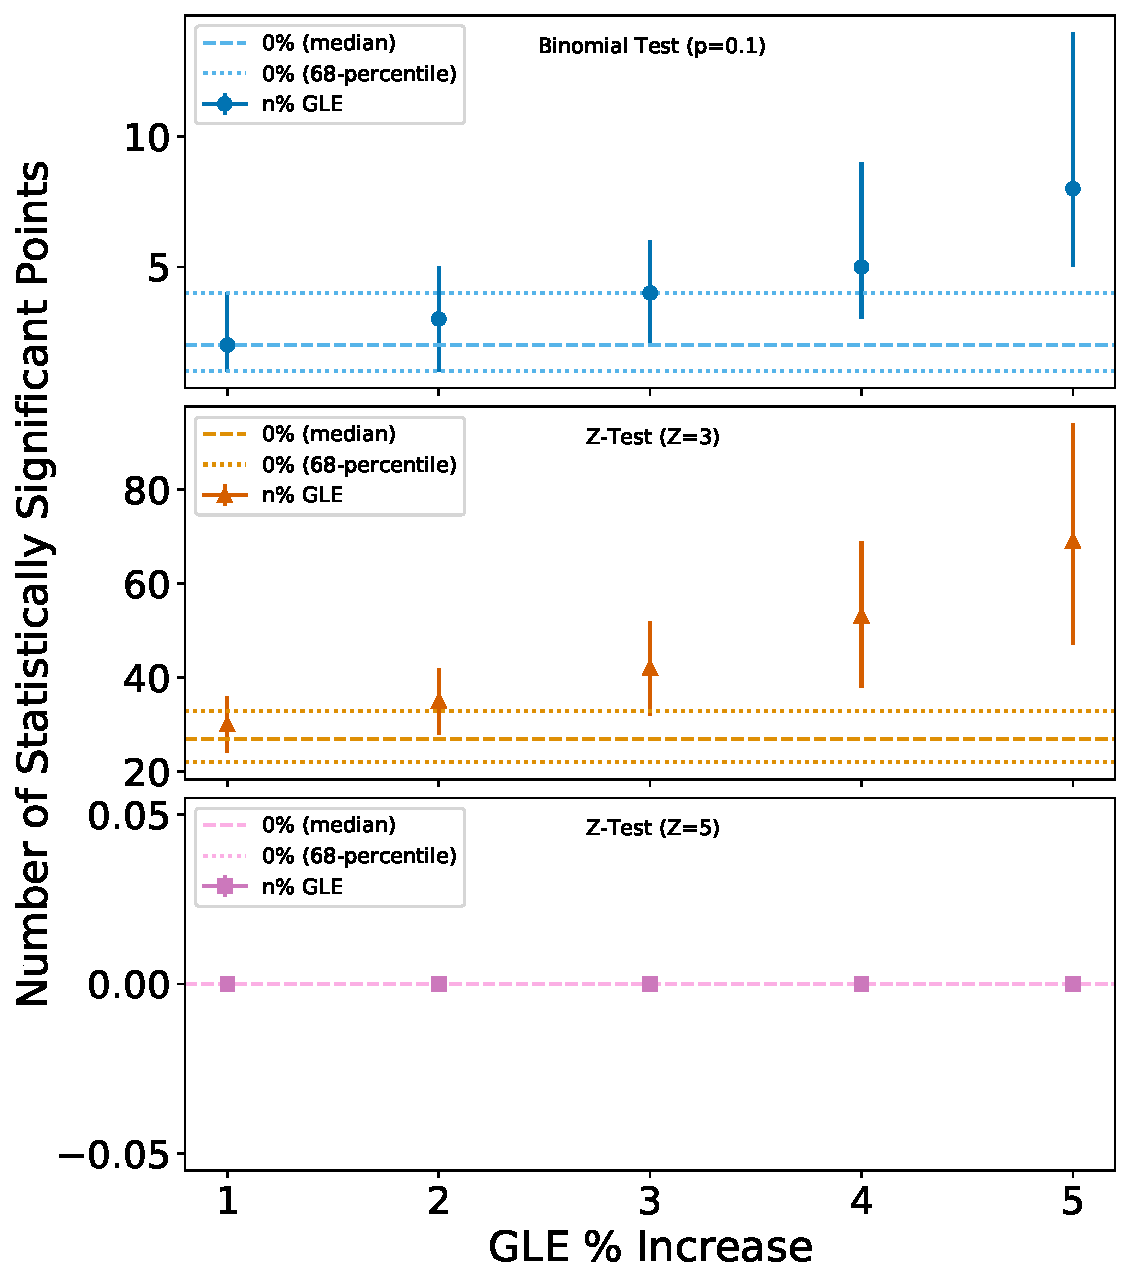
\includegraphics[width=0.48\columnwidth]{HS_14008_sims_plot_1stn.pdf}
		\label{fig:multi_sims_1stn}}
	%\qquad
	\subfloat[2 stations]{
		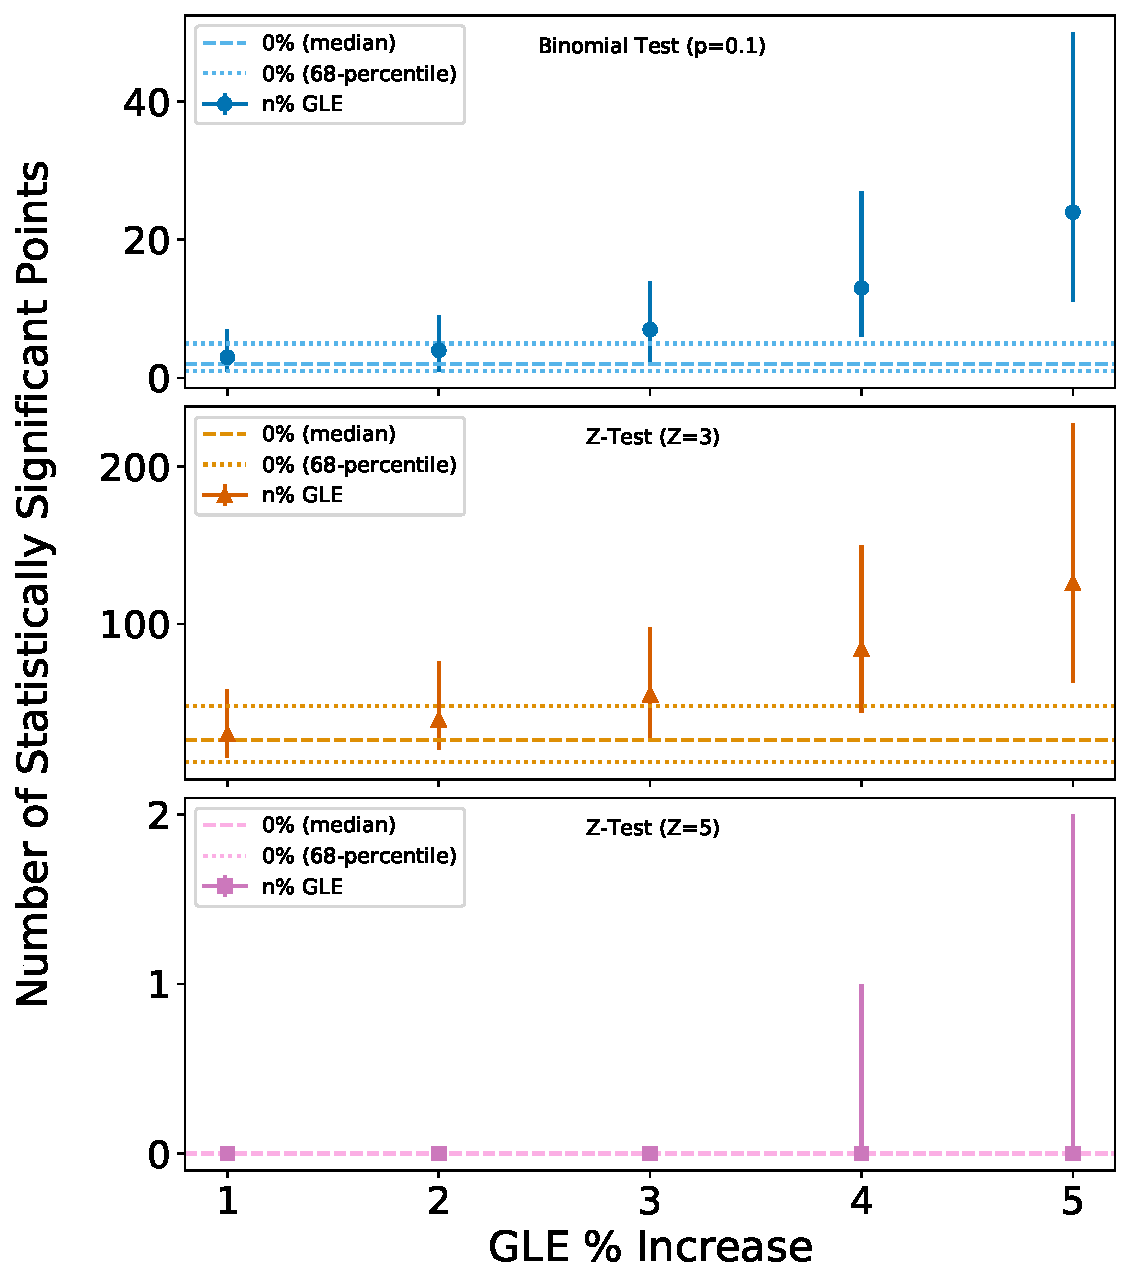
\includegraphics[width=0.48\columnwidth]{HS_14008_sims_plot_2stn.pdf}
		\label{fig:multi_sims_2stn}} \\
	%\qquad
	\subfloat[5 stations]{
		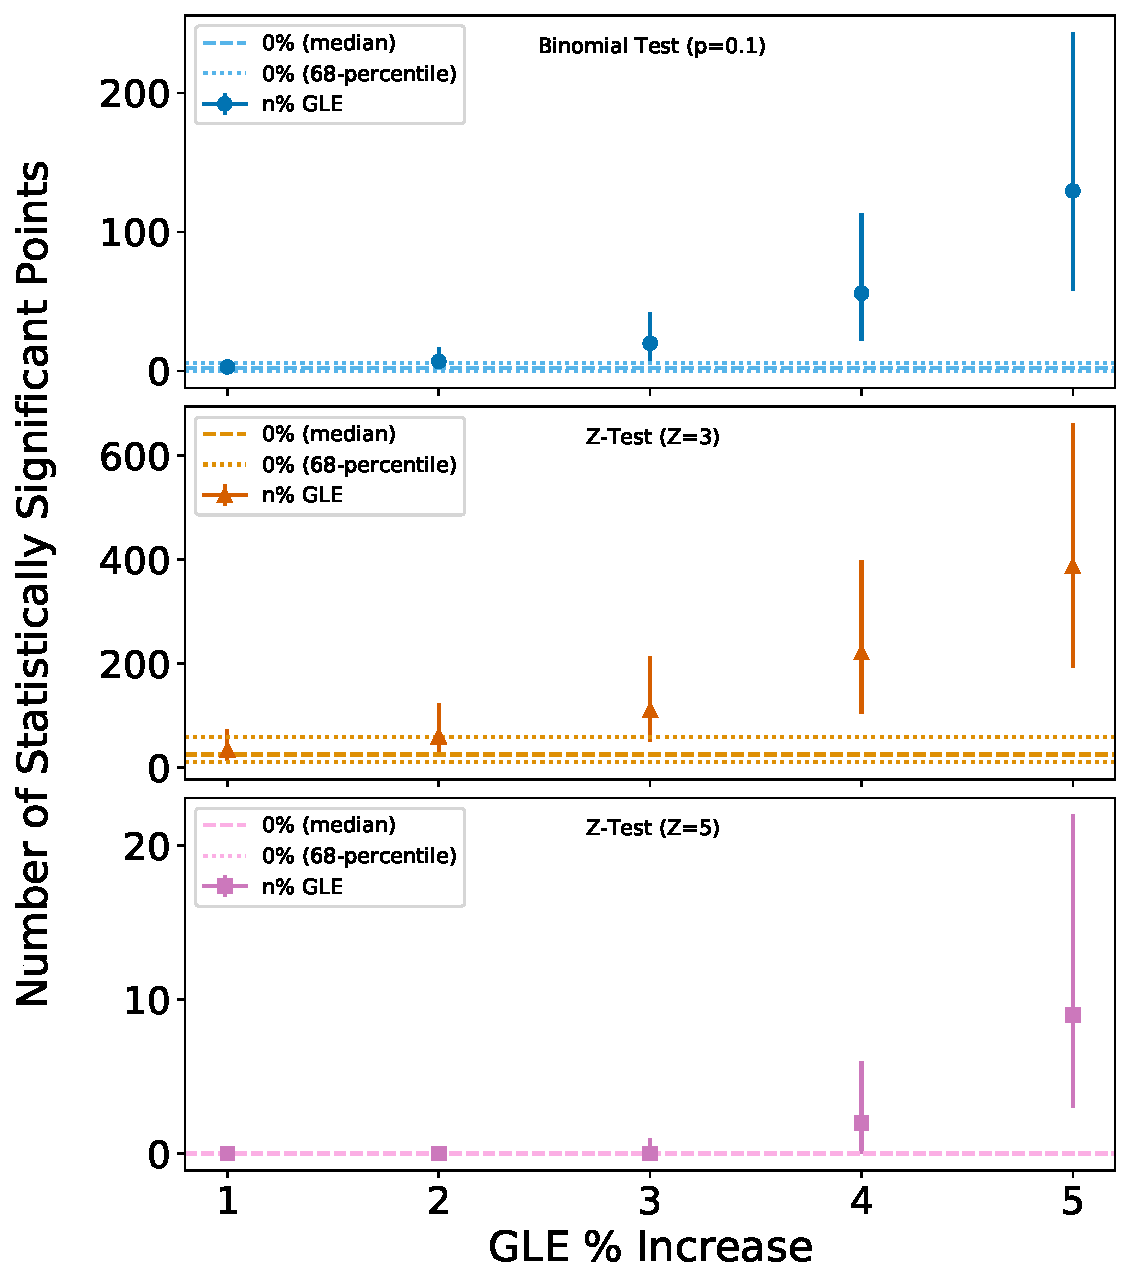
\includegraphics[width=0.48\columnwidth]{HS_14008_sims_plot_5stn.pdf}
		\label{fig:multi_sims_5stn}} 
		%\qquad
	\subfloat[10 stations]{
		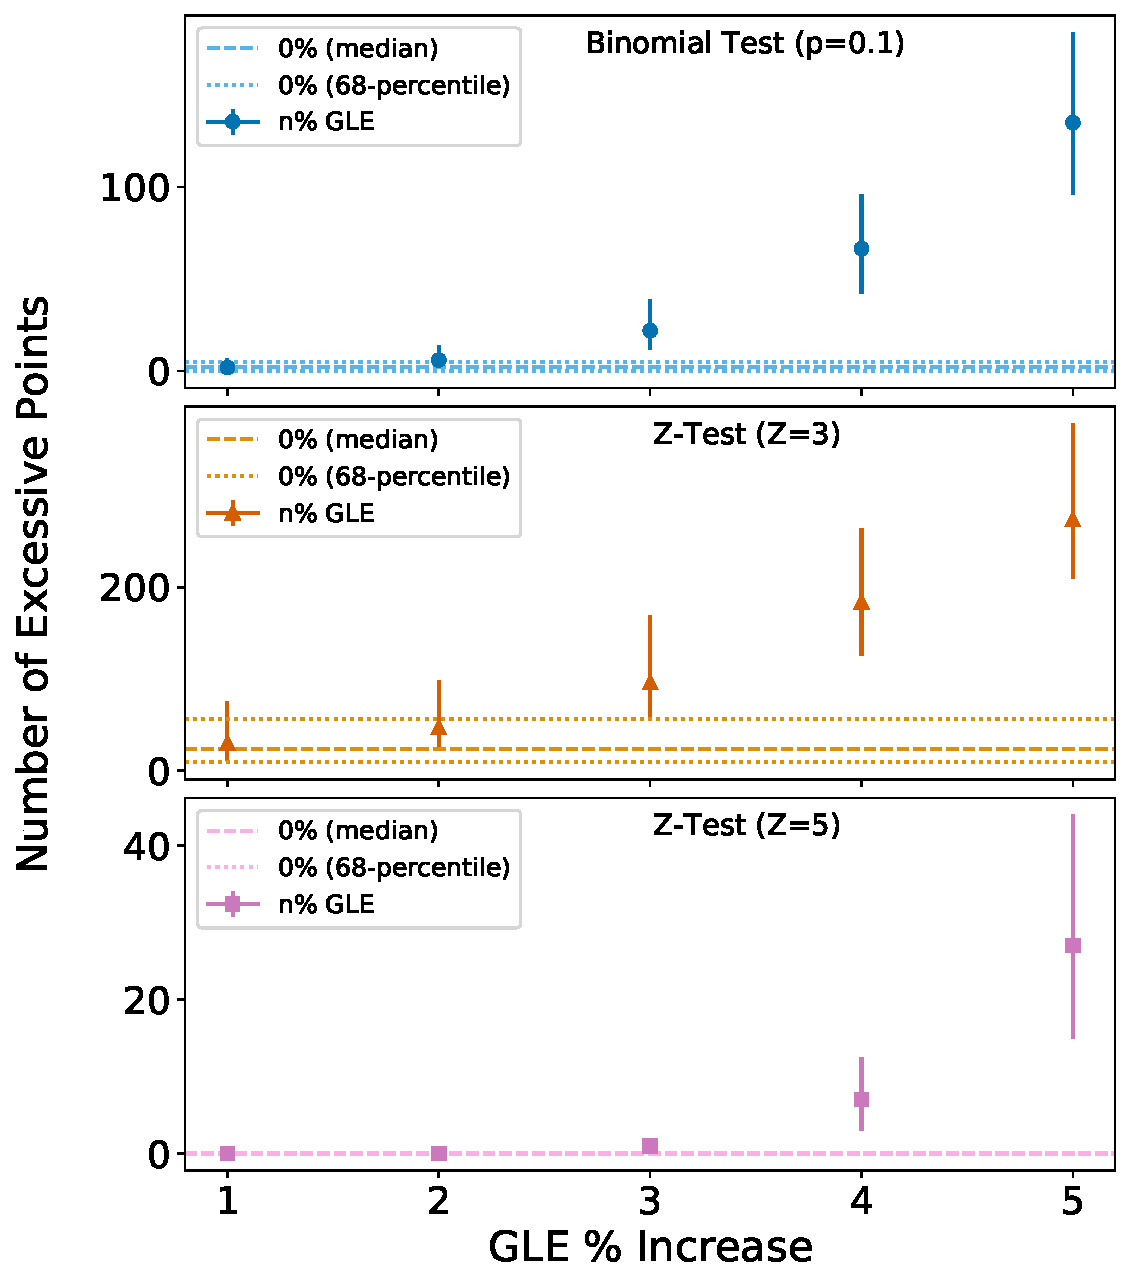
\includegraphics[width=0.48\columnwidth]{HS_14008_sims_plot_10stn.pdf}
		\label{fig:multi_sims_10stn}} \\
	
	\caption{Summary plots showing the number of statistically significant measurements using the binomial- and Z-tests on the simulations of artificial data with varying magnitudes of GLEs injected. (a) ...; (b) ...; (c) ...; (d) ... . In each plot, the top panel shows the number of significant points exceeding the binomial $p = 10 \%$ threshold, the middle panel shows the number of points exceeding the Z=3 threshold, and the bottom panel shows the number of points exceeding the Z=5 threshold. The dashed, horizontal lines show the median values of the tests without an injected GLE, and the horizontal, dotted lines represent the $68 \%$ credible intervals either side of the median. For each simulated GLE magnitude the point represents the median values and the error bars represent the $68 \%$ credible intervals either side of the median.}
	\label{fig:multi_HS14008_sims}
\end{figure}

[discussion and plots on increasing the number of stations for different GLE magnitudes... need a summary plot to show this, i.e. stats test on the average timeseries for 2, 5, 10 stations (also show single stations from above!!)...]

[discussion on the spread being a side-effect of the randomly sampled rise and decay, allowing for more measurements to remain above the threshold for longer if a longer decay...]

In addition, we also perform cross-correlation analyses between the multiple stations simulated. This again relies on the assumption that the signal registered at each station has minimal delay, such that the peak of the \gls{ccf} is at a time shift of zero. This analysis was performed for simulations of 2, 5, and 10 stations, with varying lengths of the \gls{gle} decay, to also investigate the effect that this has on our ability to detect the event using this method.

[Section on CCF and need to show how the effects of varying the decay time varies the ability to observe - also show how ability to claim varies with number of stations used... this is for 2 per cent GLE...]


\begin{figure}[ht!]
	\centering
	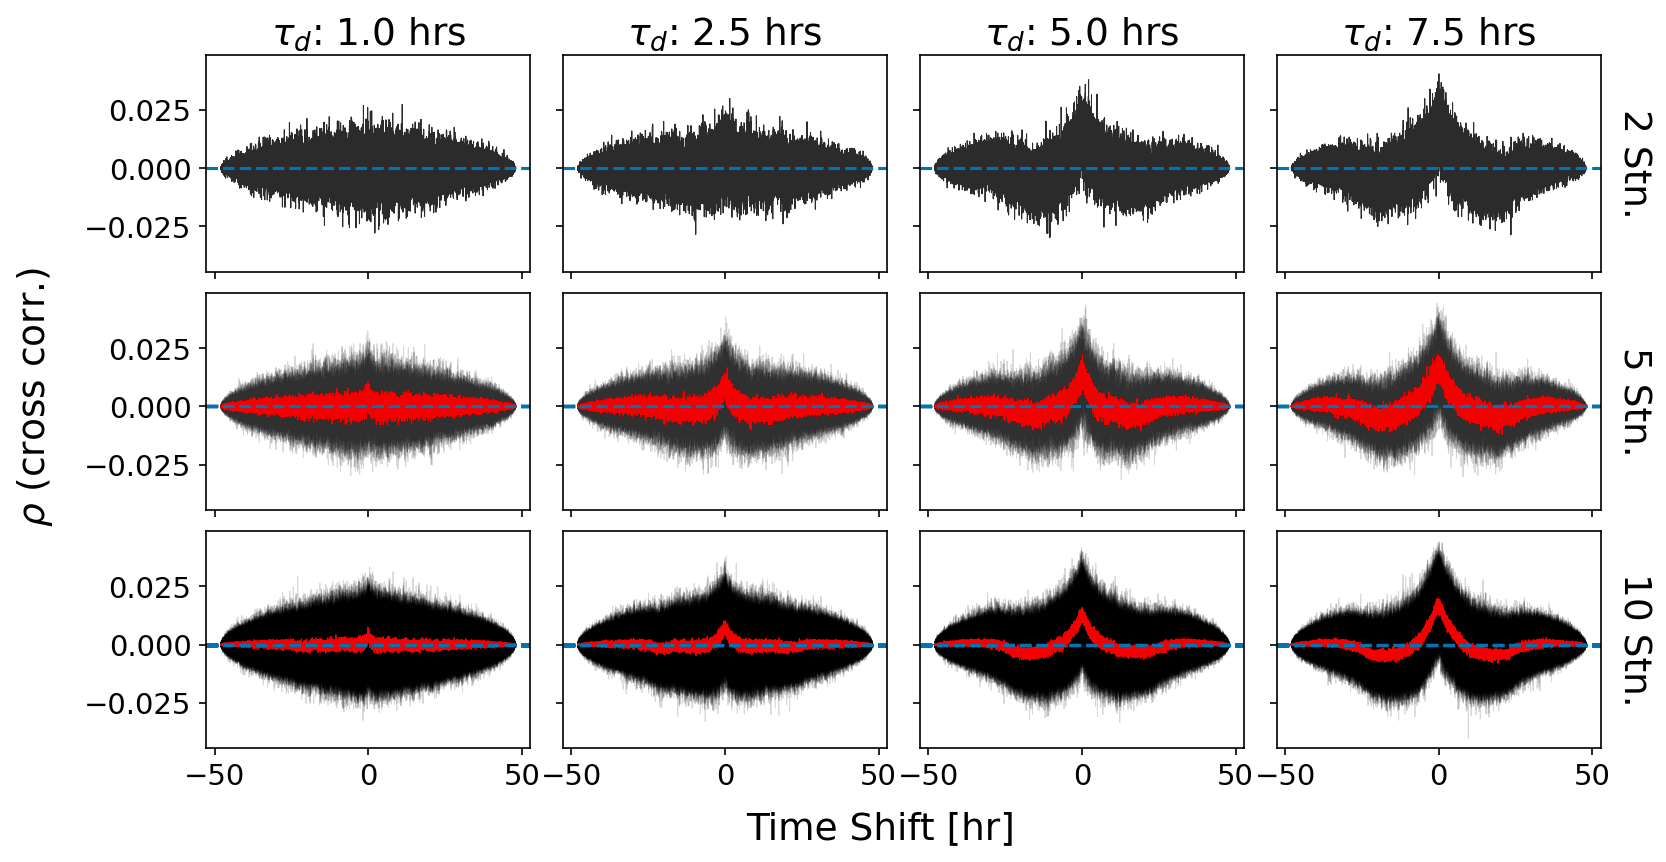
\includegraphics[width=\columnwidth]{HS_14008_sims_CCF_2pc_plot.png}
	\caption{... for $2\%$ GLE magnitude ...}
	\label{fig:HS_14008_2pc_sim_CCFs}
\end{figure}




We see from Figure... that increasing the number of stations means we can average over the \glspl{ccf} which results in a less-noisy \gls{ccf}. This is advantageous as it allows us to more clearly detect the correlated signals between 5 and 10 stations, versus with only 2 stations... There is not a significant benefit at this level of \gls{gle} in increasing from 5 to 10 stations. However, the benefit of an increased number of stations is that we are able to reduce the noise on the combined signal, which allowed us to observe significant peaks in the statistics tests (in earlier fig...)...

[Also show CCF for 1 per cent GLE with varying the number of stations (do we also want to show the varying of the decay time too? basically a repeat of the above plots but for 1 per cent GLE???)]

\begin{figure}[ht!]
	\centering
	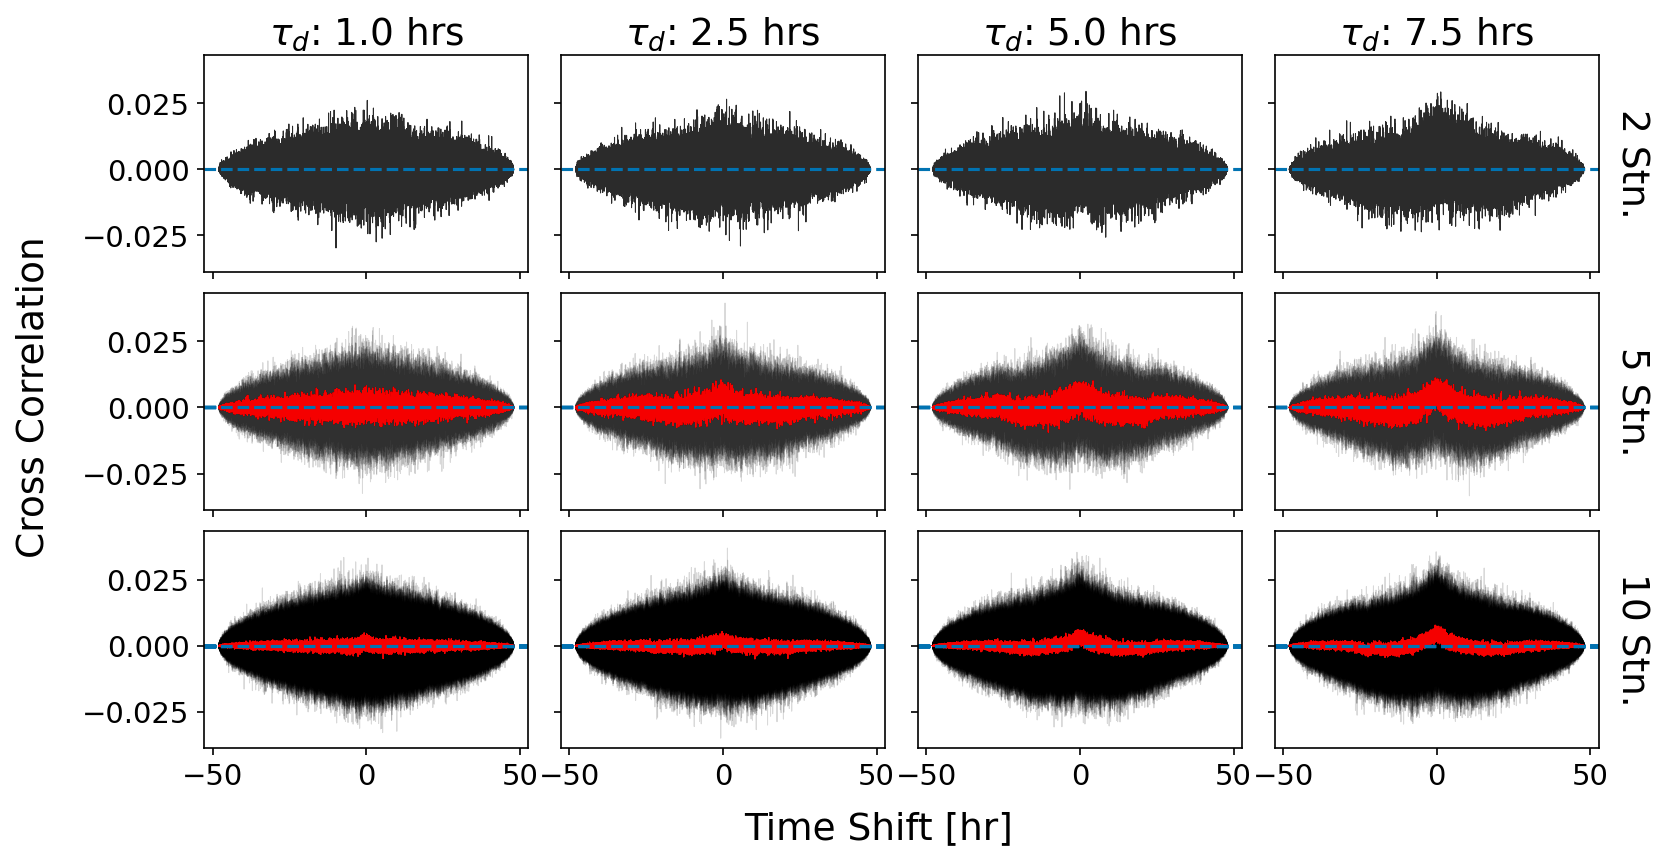
\includegraphics[width=\columnwidth]{HS_14008_sims_CCF_1pc_plot.png}
	\caption{... for $1\%$ GLE magnitude ...}
	\label{fig:HS_14008_1pc_sim_CCFs}
\end{figure}




[Do we mention PCA??? maybe no...]

[conclusive statements... how many stations do we think should be changed?]


%%%%%%%%%%%%%%%%%%%%%%%%%%%%%%%%%%%%%%%%%%%%%%%%%%%%%%%%%%%%%%%%%%%%%
%%%%%%%%%%%%%%%%%%%%%%%%%%%%%%%%%%%%%%%%%%%%%%%%%%%%%%%%%%%%%%%%%%%%%
\section{Conclusions}\label{sec:HS_14008_conclusion}

We have presented a new \gls{hisparc} station configuration and investigated its performance as a monitor of space weather events...

...

...


We leave the reader with the following points:

\begin{enumerate}
	\item{}

	\item{}
	
	\item{}
	
	\item{... It is therefore important that this configuration of \gls{hisparc} detector is maintained until at least 2026, to ensure a complete study is performed.}
\end{enumerate}